\chapter{A construção da integração mundial}
\markboth{Módulo 1}{}

%\reduline{Este módulo foi estruturado seguindo uma linha temporal que explicita o desenvolvimento do processo de globalização e, ao mesmo tempo, mobiliza os conteúdos necessários para a efetivação do eixo e das habilidades associadas.}

<<<<<<< HEAD
\section{Habilidades da BNCC}

\begin{itemize}
  \item 
EF09GE05, EF09GE06, EF09GE09.
\end{itemize}

=======
>>>>>>> 92e3cd6407615258ebd886843e38a91cbf55d87c
\section{Eixo de conhecimento do SAEB}

\begin{itemize}
\item Tempo e espaço: fontes e formas de representação
\end{itemize}

\conteudo{O desenvolvimento da configuração de mundo atual é resultado de longo processo histórico, que não pode ser compreendido sem considerarmos o papel da colonização e do desenvolvimento do capitalismo, sistema econômico que hoje integra todo o mundo em sua lógica.

Tal processo possui íntima relação com o desenvolvimento da cartografia, que, desde suas bases na Antiguidade, desenvolveu-se seguindo os rumos das grandes navegações, o que torna evidente também quanto a Antiguidade Clássica relaciona-se com a Europa que colonizou o mundo.

A globalização integrou o mundo por meio do desenvolvimento tecnológico e da consolidação do capitalismo a nível global, conseguindo estabelecer padrões gerais de consumo, cultura e organização social. Tal interação assenta-se no predomínio das lógicas ocidentais do mundo gestadas na Europa.}

%\reduline{Ao longo das atividades, ficará perceptível que as questões estão encadeadas, de modo que o conteúdo vai se articulando por meio de atividades interpretativas que mobilizam também o conteúdo previsto para ser visto ao longo dos quatro Anos Finais do Ensino Fundamental. Essa é uma forma que facilita a compreensão do aluno ao seguir uma estrutura que remete a uma sequência de aulas.}


\section{Atividades}

\begin{quote}
Os mapas medievais ``T e O'' originaram-se da descrição do mundo na
obra \emph{Etymologia}, de Isidoro de Sevilha. Este conceito de
cartografia medieval representa apenas o hemisfério norte de uma Terra
esférica, dedução feita a partir da projeção da porção habitada do mundo
conhecida nos tempos romanos e medievais.

\begin{figure}[htpb!]
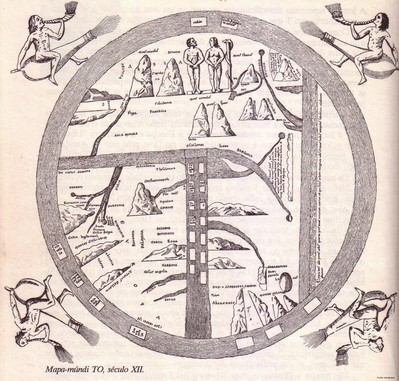
\includegraphics[width=2.88577in,height=2.76032in]{./imgs/img1.jpg}
\caption{Fonte: /www.geografia.seed.pr.gov.br/modules/galeria/detalhe.php?foto=401\&evento}
\end{figure}

O ``T'' é o Mediterrâneo
dividindo em três contimentes: Europa, Ásia e África, sendo o ``O'' um
Oceano circundante. Jerusalém era usualmente representada no centro do
mapa e a Ásia surgia do tamanho da soma dos outros dois continentes.
Porque o Sol nascia a leste, e o Paraíso (jardim do Éden) era geralmente
representado como sendo na Ásia, estando, dessa maneira, situada na
porção superior do mapa.

\fonte{Secretaria da Educação. Mapa T O. Disponível em: \emph{www.geografia.seed.pr.gov.br/modules/galeria/detalhe.php?foto=401\&evento}. Acesso em: 19 fev. 2023.}
\end{quote}

\num{1} Mapas são representações não apenas do espaço geográfico, mas também
de ideias e concepções de mundo. No caso do mapa T O, qual era a
concepção de mundo em sua base?


\reduline{Como o mapa representava apenas a porção do planeta conhecida pelos
elaboradores, a concepção de mundo deles acreditava que não existia mais
superfície terrestre para além das áreas conhecidas, sendo esse conjunto
o único tipo de mundo aceito como existente.\hfill}
\linhas{2}

\num{2} O mapa T O era um mapa medieval, de uma época em que não estavam prontas as
bases da cartografia como a conhecemos hoje. Circule os nomes dos elementos que estão ausentes nesse mapa, mas que devem
\textbf{obrigatoriamente} existir nos mapas contemporâneos.

\begin{multicols}{2}
\red{LEGENDA}

FIGURAS

\red{TÍTULO}

SIMBÓLICAS

TRAÇADO DE ESTRADAS
\end{multicols}

%\reduline{Os mapas contemporâneos precisam dispor de alguns elementos básicos, como título, legenda, escala e orientação. Esses elementos permitem identificarmos o tema, como ele está sendo representado, comparação entre o tamanho do mapa e o tamanho da área representada e a disposição dos elementos espaciais no espaço.}

\num{3} Leia os dois textos a seguir.

\textbf{TEXTO 1}
\begin{quote}

{[}...{]}

Durante muitos séculos, os mapas foram um privilégio da elite.
Apenas reis, nobres, alto clero, grandes navegadores e armadores de
expedições marítimas, tinham acesso a esse tipo de informação. Somente a
partir da invenção da imprensa, na segunda metade do século XV, os mapas
puderam ser mais amplamente utilizados.

{[}...{]}

\fonte{IBGE. \emph{Atlas Geográfico Escolar na
Internet.} Disponível em:
\emph{https://atlasescolar.ibge.gov.br/conceitos-gerais/historia-da-cartografia/a-era-dos-descobrimentos-sec-xv-a-xviii.html}.
Acesso em: 19 fev. 2023.}
\end{quote}

\textbf{TEXTO 2}
\begin{quote}

Depois de inventar os tipos móveis, Gutenberg ajudou a dar início
a uma revolução cultural. Os padrões de impressão definidos por ele
consolidaram-se de tal forma que se mantiverem sem grandes alterações
até o século XVIII. Por isso, o nome de Gutenberg está na lista dos
personagens mais influentes da história. Em 2000, por exemplo, alguns
meios de comunicação o definiram como o \textbf{homem do milênio}.

\fonte{Fonte de pesquisa: National Geographic Portugal. Johannes Gutenberg e os princípios da impressão. Disponível
em: \emph{https://nationalgeographic.pt/historia/grandes-reportagens/3086-johannes-gutenberg-e-os-principios-da-impressao}.
Acesso em: 19 fev. 2023.}
\end{quote}

Agora, leia esta afirmativa:

\begin{quote}
\textit{A popularização e o aperfeiçoamento dos mapas estão diretamente relacionados
ao avanço técnico ocorrido às vésperas do mercantilismo.}
\end{quote}

Explique se você concorda com essa afirmativa ou se você discorda dela.


\reduline{A articulação entre os textos deixa claro que os mapas deixaram de ser
privilégio da elite apenas após a capacidade de impressão em massa dos
mapas ser atingida, ou seja, temos uma inovação técnica associada ao
desenvolvimento cartográfico.\hfill}
\linhas{2}

\num{4} Leia o texto.

\begin{quote}
\textbf{Mercantilismo}

{[}...{]}

A obtenção de riqueza no mercantilismo poderia se dar de diversas
maneiras. O Estado poderia cobrar impostos da população, vender cargos
públicos e títulos de nobreza, confiscar bens, ceder privilégios
comerciais para um determinado grupo em troca de compensação financeira
(monopólios), exportar mercadorias, saquear em contextos de guerra,
cobrar taxas alfandegárias, realizar ações de pirataria
etc.

{[}...{]}

Um acontecimento extremamente importante para o sucesso
dessas práticas econômicas entre as nações europeias foi o
colonialismo.

O colonialismo foi fundamental para os Estados europeus, pois
permitiu que eles explorassem inúmeros recursos de suas colônias e os
enviassem para a Europa. Isso também possibilitou que essas colônias
fossem transformadas em consumidores compulsórios de suas metrópoles,
por conta do exclusivismo comercial.

{[}...{]}

\fonte{Daniel Neves Silva. História do Mundo. Mercantilismo. Disponível em:
\emph{https://www.historiadomundo.com.br/idade-moderna/mercantilismo.htm}.
Acesso em: 19 fev. 2023.}
\end{quote}

Na Idade Média, considerava-se o mundo como
restrito a Europa, Ásia e África. A partir da leitura do texto, o que
muda na visão europeia sobre a extensão do mundo a partir do
mercantilismo?


\reduline{Em contraposição à ideia de um mundo restrito a Ásia, Europa e África, a
colonização marcou também a ``descoberta'' do continente americano pelos
europeus, o que ampliou o mundo conhecido até então.\hfill}
\linhas{2}

\num{5} A globalização é caracterizada pela integração de fluxos comerciais,
populacionais, culturais e sociais. Sobre o assunto, analise estas informações:

\begin{itemize}
  \item \textbf{1500-1840}: a velocidade média das carruagens e dos barcos a vela
  era de 16 km/h;
  \item \textbf{1850-1930}: a velocidade média das locomotivas a vapor era de 100 km/h,
  enquanto a dos barcos a vapor era de 57 km/h;
  \item \textbf{Década de 1950}: os jatos de passageiros alcançavam velocidades entre
  480 e 640 km/h;
  \item \textbf{Década de 1960}: os jatos de passageiro alcançavam velocidades entre
  800 e 1.100 km/h.
\end{itemize}

Como essas informações relacionam-se com a globalização?


\reduline{Com o passar do tempo, os meios de transporte se desenvolveram, o que diminuiu
os tempos de locomação entre dois pontos do mundo, como se as distâncias no planeta tivessem
também diminuído. Com isso, veio a maior rapidez nos deslocamentos de pessoas e mercadorias,
uma característica da globalização.\hfill}
\linhas{2}

\num{7}

\begin{quote}
\textbf{Globalização}

{[}...{]}

A origem dos termos \emph{sociedade global}
e \emph{globalização} é anterior ao triunfo político
da \emph{globalização neoliberal}; data
de finais dos anos 1960 e deve ser creditada a MacLuhan e a Bzezinski
{[}...{]}. {[}...{]} Brzezinski colocou em circulação as expressões \emph{cidade global} e
\emph{sociedade global} para designar a nova reconfiguração globalizada do
nosso hábitat, operada pelas redes tecnotrônicas (termo introduzido por
ele para designar a conjugação do computador, da TV e da rede de
telecomunicação). O protótipo dessa ``sociedade global'' eram os [Estados Unidos],
centro propulsor da revolução ``tecnotrônica'' mundial que oferecia ao
mundo o ``único modelo global de modernidade'', com os correspondentes
``padrões de comportamento e valores universais''.

{[}...{]}

\fonte{Ramon Peña Castro. Dicionário da
educação profissional em saúde. Globalização. Disponível em:
\emph{http://www.sites.epsjv.fiocruz.br/dicionario/verbetes/glo.html}.
Acesso em: 19 fev. 2023.}
\end{quote}

Segundo o texto, como o advento de novas tecnologias de comunicação
ajudou a integrar o conjunto dos países?


\reduline{Os meios de comunicação tornam possível a transmissão de informações
para lugares distantes, e não apenas informação, mas também ideias,
modelos de vida e manifestações culturais. Quem domina os meios de
comunicação também domina o que é transmitido, ajudando a moldar os
discursos dominantes.\hfill}
\linhas{2}

\num{8} Leia o texto.

\begin{quote}
\textbf{Saiba um pouco mais sobre a história do movimento Manguebeat}

O manguebeat surgiu em Pernambuco, como um movimento de
contracultura. Ele era formado principalmente por jovens que usavam a
música como uma forma de inclusão social {[}...{]}.

O nome surgiu de uma fusão da palavra \emph{mangue} com a palavra \emph{bit}
(unidade de memória de computadores). Assim como o mangue, que é rico em
sua biodiversidade, o manguebeat criou uma cena musical bem
diversificada, misturando ritmos regionais pernambucanos como: maracatu,
frevo, ciranda e caboclinho, pop, rap, hip hop e música eletrônica. O
movimento se beneficiou de ferramentas tecnológicas recém-surgidas, o
que proporcionou a gravação das músicas em ``home studios'', e do
surgimento da internet, principal fonte de divulgação.

Diversos grupos se destacaram: Mundo Livre S/A, Chico Science \&
Nação Zumbi, Sheik Tosado, Mestre Ambrósio, Faces do Subúrbio, Eddie,
Via Sat, Querosene Jacaré e Jorge Cabeleira.

{[}...{]}

\fonte{TV UNESP. Saiba um pouco mais sobre a história do movimento Manguebeat.
Disponível em: \emph{https://tv.unesp.br/old/616}. Acesso
em: 19 fev. 2023.}
\end{quote}

Músicas como pop, rap e eletrônica possuem origens diversas para além das
fronteiras brasileiras. Nesse sentido, o que a mistura desses ritmos por
grupos brasileiros pode dizer sobre a globalização?


\reduline{A fusão de ritmos demonstra que a música não se restringe mais aos
países e aos territórios em que são criadas, espalhando-se pelos meios
de comunicação, o que permite também a apropriação por outros grupos.
Isso gera uma integração cultural característica da globalização.\hfill}
\linhas{3}

\num{9} Leia as informações a seguir.

\textbf{I. Os 10 produtos mais exportados pelo Brasil em 2022 para a China}

\begin{enumerate}
\item Soja;
\item Minério de ferro e seus concentrados;
\item Óleos brutos de petróleo ou de minerais betuminosos;
\item Açúcares e melaços;
\item Carne bovina;
\item Farelos de soja e outros alimentos para animais;
\item Celulose;
\item Milho não moído;
\item Produtos manufaturados;
\item Carnes de aves e suas miudezas comestíveis, frescas, refrigeradas ou congeladas.
\end{enumerate}

\fonte{Fonte de pesquisa: Fazcomex, 22 nov. 2022. Disponível em:
\emph{https://www.fazcomex.com.br/comexstat/asia/exportacao-china/}.
Acesso em: 03 abr. 2023.}

\textbf{II. Os principais produtos importados pelo Brasil da China}

\begin{enumerate}
\item
  Equipamentos de telecomunicações;
\item
  Válvulas e tubos termiônicas;
\item
  Compostos organo-inorgânicos;
\item
  Produtos manufaturados;
\item
  Adubos ou fertilizantes;
\item
  Medicamentos e produtos farmacêuticos, exceto veterinários;
\item
  Máquinas e aparelhos elétricos;
\item
  Peças e acessórios para escritório;
\item
  Aparelhos elétricos para ligação;
\item
  Máquinas de energia elétrica;
\end{enumerate}

\fonte{Fonte de pesquisa: Fazcomex, 22 mar. 2023. Disponível em:
\emph{https://www.fazcomex.com.br/comex/produtos-importados-da-china-para-o-brasil/}.
Acesso em: 03 abr. 2023.}

\begin{escolha}
\item Quem vende mais produtos industrializados, Brasil ou China?

\reduline{A China vende mais produtos industrializados do que o Brasil.\hfill}

\item O que isso revela sobre a relação entre os dois países?

\reduline{Isso mostra que o parque industrial chinês è mais desenvolvido e que a
indústria tem menor participação na composição econômica do Brasil.\hfill}
\end{escolha}

\num{10} A produção industrial mundial concentra-se na América do Norte, no leste
da Ásia e no oeste da Europa. Sobre isso, explique o significado desta afirmativa:

\begin{quote}
A globalização é marcada por um pequeno grupo de países produtores e um
imenso grupo de consumidores.
\end{quote}


\reduline{A produção industrial é monopólio de poucos países, ou seja, eles
produzem aquilo de mais avançado existente até hoje, enquanto o restante
do mundo apenas consome os produtos e reproduzem a tecnologia fabril
oriunda de outros países.\hfill}
\linhas{3}

\section{Treino}

\num{1} Leia o texto.

\begin{quote}
\textbf{O mundo ocidental e o mundo oriental}

De modo geral, podemos definir o mundo oriental como a porção
da Terra formada pelas nações da Ásia e do Oriente Médio, enquanto o
mundo ocidental engloba a Europa e grande parte dos territórios que
foram colonizados pelos europeus, notadamente a América, a Austrália e a
Nova Zelândia.

{[}...{]}

\fonte{Conexão Escola. Prefeitura de Goiânia. Disponível em:
\emph{https://sme.goiania.go.gov.br/conexaoescola/eaja/geografia-mundo-oriental-e-mundo-ocidental/}.
Acesso em: 20 fev 2023.}
\end{quote}

Identifica-se no texto que o mundo ocidental corresponde

\begin{escolha}
\item
  ao conjunto dos países europeus.
\item
  às sociedades que seguem o Islamismo.
\item
  aos territórios localizados no Hemisfério Oeste.
\item
  aos países condicionados pela cultura europeia.
\end{escolha}


\num{2} Leia o texto.

\begin{quote}
\textbf{História da cartografia: a Idade Média}

Isodoro (570-636 d.C.), bispo de Sevilha, criou o mapa
etimologias, também conhecido como mapa T-O. Esse mapa esquemático tinha
o seguinte significado: o ``T'' representava os três cursos d'água que
dividiam o ecúmero, o Mediterrâneo, que separa a Europa da África; o
Nilo, separando a África da Ásia; e o Don, entre a Ásia e a Europa. O
ecúmero teria sido dividido por Noé entre seus três filhos após o
dilúvio. Além disso, o ``T'' também simbolizava a cruz e na sua junção
estaria localizada Jerusalém, centro do mundo. Esses mapas, em sua
maioria, eram circulares e emoldurados por um grande oceano.

{[}...{]}

\fonte{IBGE. Atlas escolar. Disponível em:
\emph{https://atlasescolar.ibge.gov.br/conceitos-gerais/historia-da-cartografia/a-idade-media.html}.
Acesso em: 20 fev. 2023.}
\end{quote}

A concepção de um mundo restrito a Europa, Ásia e África representada
nos mapas T-O explica-se

\begin{escolha}
\item
  pelo restrito conhecimento astronômico.
\item
  pela inexistência de satélites que fotografassem do espaço.
\item
  pelo desconhecimento de outros locais por parte dos europeus.
\item
  pela crença de existência em um mundo habitado por seres míticos.
\end{escolha}

\num{3} Leia o texto.

\begin{quote}
\textbf{Fórum Social Mundial}

Conforme define sua Carta de Princípios, o Fórum Social Mundial
é um espaço internacional para a reflexão e organização de todos os que
se contrapõem à globalização neoliberal e estão construindo alternativas
para favorecer o desenvolvimento humano e buscar a superação da
dominação dos mercados em cada país e nas relações internacionais.
{[}...{]}

\fonte{Espaço Fórum Social Mundial Porto Alegre. Fórum Social Mundial. Disponível em:
\emph{http://forumsocialportoalegre.org.br/forum-social-mundial/}. Acesso
em: 20 fev. 2023.}
\end{quote}

A justificativa apresentada pelo texto valida a ideia de que a
globalização seria um sistema mundial baseado

\begin{escolha}
\item
  na integração dos sistemas políticos nacionais.
\item
  na solidariedade mútua entre a comunidade global.
\item
  no desenvolvimento pleno dos antigos países colonizados.
\item
  no domínio territorial por parte dos mercados desenvolvidos.
\end{escolha}


\chapter{Energia e circuitos produtivos}
\markboth{Módulo 2}{}

%\reduline{Este módulo parte do entendimento do conceito de energia para embasar um raciocínio que sintetiza como ocorre o intermédio da relação sociedade-natureza por meio de seus circuitos que exploram os recursos naturais. O mesmo conceito serve de alicerce para a compreensão dos fenômenos naturais e sua relação com as intervenções humanas na paisagem. Três pontos são fundamentais para o trabalho pedagógico deste módulo, que se resumem ao entendimento das Revoluções Industriais como um processo com o qual se complexificaram as tecnologias de produção de energia e de produção industrial, o que resultou na criação de estruturas urbanas que centralizavam cada vez mais a população e o funcionamento econômico. Essa concepção é necessária para que os alunos consigam compreender e resolver as primeiras atividades. 

\section{Habilidade da BNCC}

\begin{itemize}
  \item 
EF09GE18.
\end{itemize}

\section{Eixo de conhecimento do SAEB}

\begin{itemize}
\item Natureza e questões socioambientais.
\end{itemize}

\conteudo{Não conseguimos compreender a atual configuração do mundo globalizado e todos os seus problemas e desafios sem considerarmos o papel da industrialização de base ocidental na conformação desse mundo, sendo a urbanização contemporânea filha legítima das Revoluções Industriais.

Esse foi o mesmo processo que gerou um desequilíbrio entre a exploração dos recursos naturais e o tempo de renovação da natureza, demandando um direcionamento da energia para a produção industrial, a qual exige a completa desestruturação das reservas materiais da natureza.

A transferência da energia armazenada na natureza para a atmosfera gerou e gera, por sua vez, profundas alterações no ciclo climático, o que mudou os rumos dados pela natureza à superfície terrestre.

Por fim, a industrialização a nível global provocou a paulatina alienação do conjunto da sociedade de sua base natural, sendo necessária a reavaliação de nossa relação com o espaço terrestre.}

\section{Atividades}

\num{1} Observe os detalhes da imagem a seguir.

\begin{figure}[htpb!]

\includegraphics[width=\textwidth]{./imgs/img5.jpg}
%\caption{Fonte: https://pt.wikipedia.org/wiki/Revolu\%C3\%A7\%C3\%A3o\_Industrial\#/media/Ficheiro:Griffiths'\_Guide\_to\_the\_iron\_trade\_of\_Great\_Britain\_an\_elaborate\_review\_of\_the\_iron\_(and)\_coal\_trades\_for\_last\_year,\_addresses\_and\_names\_of\_all\_ironmasters,\_with\_a\_list\_of\_blast\_furnaces,\_iron\_(14761790294).jpg. Paisagem inglesa da década de 1870.}
\end{figure}

\begin{escolha}
\item Como podemos relacionar as chaminés à poluição da natureza?

\reduline{As chaminés emitem fumaça oriunda da queima de combustíveis e leva para a
atmosfera substâncias que podem intoxicar seres humanos e bichos, além de
emitir gases que modificam o funcionamento da atmosfera, como o dióxido de carbono.\hfill}

\item Que tipo de energia é utilizada nessas fábricas: fóssil, solar, hidráulica ou eólica? Explique.

\reduline{A Primeira Revolução Industrial pautou-se pela queima do
carvão mineral, um combustível fóssil, originado da mineralização de
restos vegetais. Sua queima esquentava a água para gerar vapor capaz de
mover máquinas rudimentares.\hfill}
\end{escolha}

\num{2} Ainda sobre a imagem presente na atividade anterior, percebe-se, na paisagem retratada, a existência de elementos rurais ao lado das fábricas.
Sobre esse fato, analise as afirmativas e marque V para o que for verdadeiro e F para o que for falso.

\begin{boxlist}
\boxitem{V} As cidades industriais intensificaram a transformação da natureza e do meio rural.

\boxitem{V} O surgimento das indústrias centralizou a economia nas cidades.

\boxitem{F} A presença de fazendas nas cidades exemplifica o convívio duradouro entre os tipos de produção.

\boxitem{F} A natureza repõe seus recursos mais rápido do que a necessidade industrial.
\end{boxlist}

%\reduline{A urbanização praticamente eliminou as atividades rurais dos centros urbanos, concentrando-as na zona rural. A produção industrial demanda recursos em uma velocidade superior àquela em que natureza os produz -- o carvão, por exemplo, leva ao menos 400 milhões de anoa para se formar e pode ser esgotado em algumas décadas.}

\num{3} Leia o texto a seguir.

\begin{quote}
\textbf{O que é energia}
Apesar de ser usada em vários contextos diferentes, o uso
científico da palavra \emph{energia} tem um significado bem definido e preciso:

Potencial inato para executar trabalho ou realizar uma ação.

Qualquer
coisa que esteja trabalhando, movendo outro objeto ou aquecendo-o, por
exemplo, está gastando (transferindo) energia.

{[}...{]}

\fonte{Eletronuclear. O que é energia. Disponível em:
\emph{www.eletronuclear.gov.br/Sociedade-e-Meio-Ambiente/Espaco-do-Conhecimento/Paginas/O-que-e-Energia}.
Acesso em: 26 fev. 2023.}
\end{quote}

Com base no texto, cite ao menos três situações em que ocorre uso de energia em seu cotidiano.


\reduline{O aluno deve citar quaisquer situações em que ocorra uso de energia,
como atividades físicas (energia metabólica) ou funcionamento de aparelhos
elétricos e motores.\hfill}
\linhas{4}

\num{4} Para o funcionamento do corpo, também é necessário gerar energia,
que é gerada a partir dos alimentos consumidos, que costumam ser cultivados. As plantas também fazem uso de
energia, extraída principalmente da luz solar combinada com os
nutrientes absorvidos do solo.

\begin{figure}[htpb!]
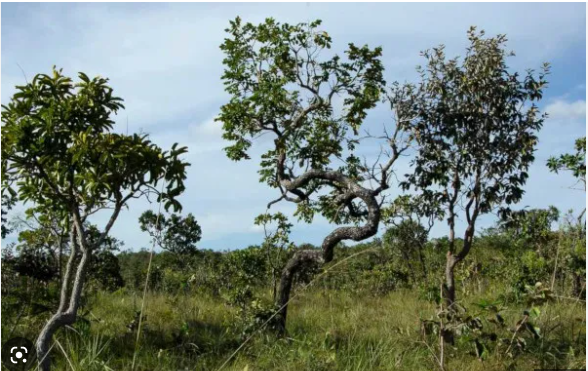
\includegraphics[width=.5\textwidth]{./imgs/img6.png}
\caption{Vegetação natural de cerrado.}

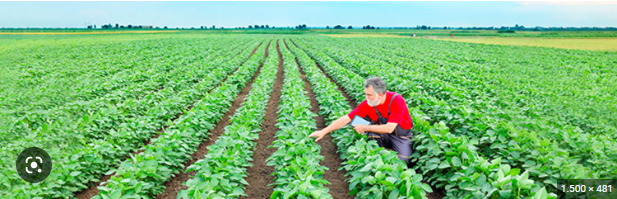
\includegraphics[width=.5\textwidth]{./imgs/img7.png}
\caption{Campo de cultivo de soja.}
\end{figure}

Considerando-se que sempre existe uma vegetação natural original onde se coloca um campo de cultivo, é correto
dizer que, na paisagem retratada na imagem em que aparece o campo de soja, há uma manipulação da energia pelo ser humano? Justifique.


\reduline{Sim. Na paisagem retratada pela primeira imagem, uma formação natural está utilizando a
energia para crescer, enquanto, na segunda paisagem, ocorreu o plantio de soja, que
também vai utilizar a energia solar para crescer, mas de uma maneira
planejada pelo ser humano.\hfill}
\linhas{5}

\num{5} Desde os alimentos que são produzidos fora da zona urbana até a própria água -- que muitas vezes é extraída longe --, as cidades dependem muito do que é externo a elas., desde os alimentos que
são produzidos fora dos limites urbanos e até da própria água, que
muitas vezes é extraída longe da cidade. A seguir, marque com um X as ações capazes
de aproximar a cidade de suas necessidades.

\begin{boxlist}
\boxitem{X} Construção de hortas urbanas.

\boxitem{} Drenagem total de rios e pântanos.

\boxitem{X} Criação de florestas urbanas.

\boxitem{} Expansão da cidade.
\end{boxlist}

%\reduline{A construção de hortas urbanas aproxima a produção de alimentos dos moradores das cidades, e as florestas urbanas promovem melhoria geral da qualidade do ar e ainda garantem a preservação de nascentes. Essas duas ações aproximariam as cidades de suas necessidades.}

\num{6} A manutenção natural do calor na atmosfera terrestre é chamada de
\textbf{efeito estufa}. O esquema a seguir ajuda a entender como se dá esse processo.

%\begin{figure}[htpb!]
%\includegraphics[width=3.07283in,height=3.91428in]%{https://br.freepik.com/vetores-gratis/o-efeito-estufa-com-luz-solar-para-casa-verde_16456035.htm#query=greenhouse%20effect&position=5&from_view=search&track=ais}
%\end{figure}

Com base nesse esquema, explique como ocorre o efeito estufa no planeta Terra.

\reduline{O efeito estufa é a retenção do calor realizada pela atmosfera terrestre e
seus componentes. A radiação solar atinge o planeta, atravessa a atmosfera, e parte, quando é refletida pela superfície, é retida pela própria atmosfera. Com isso, mantém-se o calor na superfície do planeta.\hfill}
\linhas{6}

\num{6} Leia os textos a seguir.

\textbf{TEXTO 1}
\begin{quote}
\textbf{O que é o aquecimento global?}

Trata-se do aumento da temperatura média dos oceanos e da camada de ar próxima à superfície terrestre. O aquecimento global se desenvolve conforme aumentam as emissões de determinados gases para a atmosfera -- o principal é o gás carbônico.

\fonte{Fonte de pesquisa: WWF. O que é o aquecimento global? Disponível em:
\emph{wwf.org.br/natureza\_brasileira/reducao\_de\_impactos2/clima/mudancas\_climaticas2/}.
Acesso em: 26 fev. 2023.}
\end{quote}

\textbf{TEXTO 2}
\begin{quote}
\textbf{Efeito estufa}

A queima de combustíveis fósseis (gás natural, carvão mineral e petróleo) e o desmatamento de regiões tropicais são as principais causas antropogênicas (causadas pelo ser humano) que contribuem com as emisões de gases do efeito estufa.

Os combustíveis fósseis são queimados, principalmente, pelas termelétricas, pelas indústrias e por alguns meios de transporte (automóveis, ônibus e aviões, por exemplo).

Já o desmatamento contribui com o efeito estufa porque libera as grandes reservas de carbono que as florestas representam, armazenado em biomassa florestal.

\fonte{Fonte de pesquisa: IPAM Amazônia. Quais são as principais fontes de gases de efeito estufa decorrentes das atividades humanas? Disponível em:
\emph{https://ipam.org.br/entenda/quais-sao-as-principais-fontes-de-gases-de-efeito-estufa-decorrentes-das-atividades-humanas-2/}. Acesso em: 26 fev. 2023.}
\end{quote}

Com base no texto e em seus conhecimentos, você afirmaria que o aquecimento global é a intensificação do
efeito estufa? Comente.


\reduline{O efeito estufa é um fenômeno natural importantíssimo para a manutenção da vida na Terra e é ocasionado pela presença de determinados gases na atmosfera. O problema do aquecimento global é que, com a emissão descontrolada de gases do efeito estufa, esse fenômeno intensifica-se e aquece o planeta além do necessário.\hfill}
\linhas{2}

\num{8} Os últimos trezentos anos marcaram uma profunda mudança na relação da
sociedade com a natureza, pois, a partir das revoluções
industriais, o homem passou a consumir os recursos naturais em uma
velocidade maior do que aquela com que a natureza consegue se renovar. 
Novas necessidades surgiram, e as necessidades do ser humano
passaram a ser todas intermediadas pela indústria e pautadas no
consumismo de produtos que logo são descartados. A necessidade de
produzir mais e mais implica emprego de grandes volumes de
energia, obtidos principalmente a partir da queima de
combustíveis fósseis, cuja queima emite gás carbônico, o qual intensifica a retenção de calor na atmosfera,
o que altera os ciclos naturais do clima.
Quanto a esse contexto, que alternativas o ser humano tem para não destruir seu próprio hábitat?


\reduline{Resposta pessoal. Espera-se que os alunos reflitam sobre a situação ruim em que a humanidade se encontra e tentem pensar em maneiras de alterar o quadro enquanto é tempo.\hfill}
\linhas{8}


\num{9} Indique soluções plausíveis para as causas das ilhas de calor.

\begin{escolha}
\item Excesso de construções.

\reduline{Melhoria da ventilação natural de prédios e bairros; construção de áreas de lazer abertas; investimento em arquitetura verde.\hfill}
\linhas{4}

\item Ausência de vegetação contínua.

\reduline{Reflorestamento; arborização urbana; valorização do paisagismo.\hfill}
\linhas{4}
\end{escolha}


\num{10} A vida útil média de um telefone celular é, atualmente, de dois anos, mas especialistas apontam para o fato de que, se não fosse a obsolescência programada, um celular duraria de 12 a 15 anos. Comente sobre os impactos da obsolescência programada:

\begin{escolha}
\item  na utilização de energia pelas indústrias.


\reduline{Como os produtos duram pouco, é preciso que se produza com maior
frequência, o que gera mais gasto energético.\hfill}
\linhas{3}

\item  na exploração de recursos naturais.


\reduline{A produção precisa suprir a pouca durabilidade dos produtos, e isso faz com que seja extraído da natureza um volume maior de recursos.\hfill}
\linhas{3}

\item na vida das pessoas.


\reduline{Há impacto negativo na vida das pessoas, que não conseguem realizar suas
tarefas quando os produtos estragam, além de que precisam desembolsar mais
dinheiro para garantir o acesso a itens básicos.\hfill}
\linhas{3}
\end{escolha}

\section{Treino}

\num{1} Leia o texto.

\begin{quote}
\textbf{Instalação de painéis solares cresce 560\% no País}

Que tal você mesmo gerar a energia que consome em casa, a
partir da captação da luz solar? Melhor ainda: que tal vender para a
distribuidora {[}...{]} a energia excedente? {[}...{]}

Segundo a Agência Nacional de Energia Elétrica (Aneel), nos
últimos dois anos, a instalação de painéis solares para geração própria
de energia elétrica aumentou mais de 560\%. O número saltou de 7.400
para 49 mil unidades em todo o Brasil. São instalações em residências,
empresas e indústrias.

{[}...{]}

\fonte{Jornal da USP. Instalação de painéis solares cresce 560\% no País.
Disponível
em: \emph{https://jornal.usp.br/atualidades/instalacao-de-paineis-solares-cresce-560-no-pais/}.
Acesso em: 28 fev. 2023.}
\end{quote}

O impacto ambiental do tipo de produção elétrica citado se dá em razão

\begin{escolha}
\item
  do aumento de produção de painéis.
\item
  da eliminação de redes elétricas cabeadas.
\item
  do melhor aproveitamento da energia disponível.
\item
  da diminuição do consumo total de energia elétrica.
\end{escolha}


\num{2} Compare as duas tabelas a seguir.

%Paulo, criar uma tabela com estes dados:
%Título: Matriz energética mundial (2020)
%Carvão mineral 26,8%
%Petróleo e derivados 29,5%
%Gás natural 23,7%
%Nuclear 5,0%
%Hidráulica 2,7%
%Biomassa 9,8%
%Outras 2,5%
%Fonte de pesquisa: Empresa de Pesquisa Energética. Disponível em: https://www.epe.gov.br/pt/abcdenergia/matriz-energetica-e-eletrica. Acesso em: 04 abr. 2023.

%Paulo, criar uma tabela com estes dados:
%Título: Matriz energética brasileira (2021)
%Carvão mineral 5,6%
%Petróleo e derivados 34,4%
%Gás natural 13,3%
%Nuclear 1,3%
%Hidráulica 11,0%
%Lenha e carvão vegetal 8,7%
%Derivados da cana-de-açúcar 16,4%
%Outras renováveis 8,7%
%Outras não renováveis 0,6%
%Fonte de pesquisa: Empresa de Pesquisa Energética. Disponível em: https://www.epe.gov.br/pt/abcdenergia/matriz-energetica-e-eletrica. Acesso em: 04 abr. 2023.

Observa-se que, no Brasil, a matriz energética

\begin{escolha}
\item
  segue tendências mundiais, apesar de alguns avanços.
\item
  não apresenta avanço em relação ao restante do mundo.
\item
  utiliza energia nuclear na mesma proporção que o restante do mundo.
\item
  não gera energia com base em fontes renováveis, como no restante do mundo.
\end{escolha}

\num{3} Leia o texto.

\begin{quote}
\textbf{O que são mudanças climáticas?}

As mudanças climáticas antropogênicas, ou seja, aquelas causadas
pelo homem, estão associadas ao aumento da emissão de gases de efeito
estufa por queima de combustíveis fósseis (dos automóveis, das
indústrias, usinas termoelétricas), queimadas, desmatamento,
decomposição de lixo etc. A partir do final do século 18 (Revolução
Industrial) e na segunda metade do século 20, houve uma expansão da
produção industrial, o que gerou um grande aumento de emissões de gases
de efeito estufa na atmosfera. Existem fortes indícios de que o clima
está de fato mudando. As décadas de 1990 e 2000 foram as mais quentes
dos últimos 1.000 anos. As projeções do Painel Intergovernamental de
Mudanças Climáticas (IPCC) indicam que nos próximos 100 anos poderá
haver um aumento da temperatura média global entre 1,8°C e 4,0°C, e um
aumento do nível médio do mar entre 0,18 m e 0,59 m, o que pode afetar
significativamente as atividades humanas e os ecossistemas terrestres.

\fonte{INPE. Perguntas frequentes. O que são mudanças climáticas? Disponível em: \emph{www.inpe.br/faq/index.php?pai=9\#:~:text=A\%20partir\%20do\%20final\%20do,clima\%20est\%C3\%A1\%20de\%20fato\%20mudando}. Acesso em: 28 fev. 2023.}
\end{quote}

A relação entre gases do efeito estufa e mudanças climáticas é explicada pelo fato
de as emissões humanas passarem a compor

\begin{escolha}
\item
  uma interferência dissociada dos ciclos naturais.
\item
  a capacidade de resfriamento atmosférico.
\item
  o ciclo de crescimento florestal.
\item
  o sistema climático global.
\end{escolha}

\chapter{Identidade e diversidade}
\markboth{Módulo 3}{}

\section{Eixo de conhecimento do SAEB} 

\begin{itemize}
  \item 
Culturas, identidades e diversidades.
\end{itemize}

<<<<<<< HEAD
\section{Habilidades da BNCC} 

\begin{itemize}
  \item 
EF09GE01, EF09GE02, EF09GE03, EF09HI03, EF09HI04, EF09HI26.
\end{itemize}
=======
\section{Eixo de conhecimento do SAEB} 1. Culturas, identidades e
diversidades.

\subsection{Habilidades da BNCC} 1. EF09GE01, EF09GE02, EF09GE03,
EF09HI03, EF09HI04, EF09HI26.
>>>>>>> 92e3cd6407615258ebd886843e38a91cbf55d87c

\conteudo{A cultura é um conjunto de conhecimentos, crenças, valores, tradições, costumes e práticas que são compartilhados por um grupo de pessoas e transmitidos de geração em geração. A identidade, por sua vez, refere-se ao conjunto de características que definem um indivíduo e que o distinguem dos outros, incluindo sua origem, gênero, orientação sexual, etnia, religião e outras características que compõem sua personalidade.

A diversidade cultural é a variedade de culturas e práticas que existem em todo o mundo, e que são influenciadas por diversos fatores, como a geografia, história, política e economia. A diversidade é um elemento fundamental da sociedade, pois permite a convivência pacífica entre pessoas com diferentes origens e tradições.

Nesse sentido, é importante destacar que a diversidade cultural é essencial para a compreensão e valorização das diferenças entre os indivíduos e grupos sociais, promovendo assim a tolerância e a coexistência pacífica entre eles. A valorização da diversidade e da pluralidade cultural é uma forma de construir uma sociedade mais justa, inclusiva e democrática.}

\section{Atividades}

\num{1} Leia o texto. \textgreater{}
\textbf{UE fecha acordo para proibir importação de produtos do desmatamento}
\textgreater{} Os eurodeputados chegaram {[}\ldots{}{]} a um acordo
preliminar com os governos da União Europeia sobre uma nova lei que, na
prática, vai coibir a importação pelos estados-membros do bloco de
produtos considerados --- na definição deles --- provenientes de ações
de desmatamento ilegal. A regra afirma, nesse sentido, que não serão
aceitas compras de produtos oriundos da degradação florestal de 31 de
dezembro de 2020 em diante. \textgreater{} {[}\ldots{}{]}

\fonte{Anderson Scardoelli. Canal Rural. UE fecha acordo para
proibir importação de produtos do desmatamento.
Disponível~em:~https://www.canalrural.com.br/noticias/uniao-europeia-fecha-acordo-para-proibir-importacao-de-produtos-oriundos-de-desmatamentoOs.~Acesso~em:~06~mar.~2023.}

Como a diretriz adotada pela União Europeia pode contribuir para a
redução do desmatamento ilegal?

\reduline{Devido ao comércio globalmente interligado, muitos produtos são
comercializados entre os países, e a aprovação de uma regra desse tipo
fará com que produtos que tenham se beneficiado do desmatamento deixem
de ser aceitos, o que acarretaria maior adesão às leis ambientais por
parte dos produtores.}

\num{2} Os garimpos ilegais empregam uma quantidade excessiva de
mercúrio para separar o ouro de outros sedimentos, resultando na
contaminação de peixes, destruição de rios, desmatamento e,
consequentemente, fuga da fauna. Especialistas afirmam que tudo isso
contribui para a pobreza e a propagação de várias doenças nas populações
das áreas afetadas. Esse é precisamente o caso dos habitantes da Terra
Indígena Yanomami, localizada nos estados de Roraima e Amazonas. Que
afirmativa indica o efeito da contaminação de mercúrio sobre a
comunidade Yanomami, que é uma das causas da desnutrição que afeta essa
população. Explique.

I. Baixa produção de alimentos.

\begin{enumerate}
\def\labelenumi{\Roman{enumi}.}
\setcounter{enumi}{1}
\item
  Comprometimento de práticas culturais.
\item
  Desigual distribuição da riqueza.
\end{enumerate}

\reduline{A destruição do ambiente natural é muito prejudicial aos indígenas
Yanomami, pois estes vivem de recursos disponíveis para se alimentare,
como os peixes, que acabam contaminados com o garimpo ilegal, que utiliza
substâncias tóxicas.}

\num{3} Leia o texto.

\begin{quote}
Durante muito tempo, a relação dos seres humanos com a terra e o
território não se baseava na noção de propriedade privada. Para os povos
indígenas, essa relação é ainda mais profunda, pois o território é
sagrado para eles. Como afirma Casé Angatu Xukuru Tupinambá em uma
entrevista por telefone à IHU On-Line, ``nós não somos donos da terra,
nós somos a terra''. O direito congênito, natural e originário é
anterior ao direito da propriedade privada. Em vez de lutar por reforma
agrária, os povos indígenas reivindicam o direito de estar na terra e de
proteger o que consideram sagrado: a natureza, que os nutre e é por eles
nutrida por meio da proteção.
\end{quote}

\fonte{de pesquisa: Ricardo Machado. IHU Online. ``Nós
não somos donos da terra, nós somos a terra''. Disponível em:
https://www.ihuonline.unisinos.br/artigo/7395-nos-nao-somos-donos-da-terra-nos-somos-a-terra.
Acesso~em:~07~mar.~2023.}

a) A partir do texto, como podemos diferenciar a concepção de
organização social dos indígenas frente aos colonizadores europeus?

No texto duas ideias se destacam, a de integração do homem com a Terra e
o entendimento de que a base da vida humana é natureza terrestre.

b) Em sua visão, a cultura indígena é valorizada como parte fundamental
da cultura brasileira? Por quê?

Espera-se que o aluno apresente um entendimento negativo em relação à
pergunta, demonstrando a percepção de que a cultura indígena não é de
fato valorizada pela sociedade brasileira como um todo.

\num{4} Leia o texto.

\begin{quote}
A campanha que culminou com a abolição da escravidão, em 13 de maio de
1888, foi a primeira manifestação coletiva a mobilizar pessoas e a
encontrar adeptos em todas as camadas sociais brasileiras. No entanto,
após a assinatura da Lei Áurea, não houve uma orientação destinada a
integrar os negros às novas regras de uma sociedade baseada no trabalho
assalariado.
\end{quote}

\begin{quote}
Esta é uma história de tragédias, descaso, preconceitos, injustiças e
dor. Uma chaga que o Brasil carrega até os dias de hoje.
\end{quote}

\begin{quote}
{[}...{]}
\end{quote}

\begin{quote}
A escravidão concentrava-se nas partes mais modernas da economia e
tornara-se menos relevante nos setores atrasados ou decadentes. Em 1887,
o Ministério da Agricultura, em seu relatório anual, contabilizava a
existência de 723.419 escravos no País. Desse total, a Região Sudeste
(São Paulo, Rio de Janeiro, Minas Gerais e Espírito Santo), produtora de
café, abarcava uma população cativa de 482.571 pessoas. Todas as demais
regiões respondiam por um número total de 240.848.
\end{quote}

\begin{quote}
Ao mesmo tempo, o País passara a incentivar, desde 1870, a entrada de
trabalhadores imigrantes -- principalmente europeus -- para as lavouras
do Sudeste. É um período em que convivem, lado a lado, escravos e
assalariados. Os números da entrada de estrangeiros são eloquentes.
Segundo o IBGE, entre 1871 e 1880, chegam ao Brasil 219 mil imigrantes.
Na década seguinte, o número salta para 525 mil. E, no último decênio do
século XIX, após a Abolição, o total soma 1,13 milhão.
\end{quote}

\begin{quote}
{[}\ldots{}{]}
\end{quote}

\fonte{Gilberto Maringoni. IPEA. História - O destino dos
negros após a Abolição.
Disponível~em:~\textit{www.ipea.gov.br/desafios/index.php?option=com\_content\&id=2673\%3Acatid\%3D28}.~Acesso~em:~06~mar.~2023.}

Indique as afirmativas verdadeiras sobre o período posterior à abolição
da escravidão.

( ) A população negra ganhou lotes fundiários para poder plantar.

(V) A exclusão social da população negra foi fruto da intenção de se
formar uma população brasileira ``embranquecida''.

( ) O fim da escravidão foi fator suficiente para reparar o sofrimento e
a segregação social impostos à população negra.

(V) O racismo combinado com a visão econômica colonial gerou a exclusão
social da população afrodescendente.

\num{5} Leia o texto.

\begin{quote}
A Comissão de Finanças e Tributação aprovou em dezembro o Projeto de Lei
7575/06, do Senado, que inclui quilombolas, arrendatários de terra,
produtores rurais em regime de parceria e consórcios e condomínios
agrários entre os beneficiários do crédito rural.
\end{quote}

\begin{quote}
{[}...{]}
\end{quote}

\fonte{Câmara dos deputados. Agência Câmara de Notícias.
Finanças aprova inclusão de quilombolas entre os beneficiários do
crédito rural.
\textit{Disponível~em:
www.camara.leg.br/noticias/478154-FINANCAS-APROVA-INCLUSAO-DE-QUILOMBOLAS-ENTRE-OS-BENEFICIARIOS-DO-CREDITO-RURAL}.~Acesso~em:~06~mar.~2023.}

Crédito é o nome dado a empréstimo ou condição de financiamento
oferecidos por bancos públicos ou privados. No trecho, é informado que
uma nova lei pretende aumentar a disponibilidade de crédito para a
população quilombola. Como isso afeta positivamente a participação dessa
população na atividade econômica nacional?

\reduline{Como a população quilombola é tipicamente rural, o crédito agrícola
favorece suas práticas agropecuárias, o que pode aumentar a participação
dessa população na produção agrícola nacional.}

\num{6} Leia o texto.

\begin{quote}
Os Karajá são habitantes seculares das margens do rio Araguaia,
presentes nos estados de Goiás, Tocantins e Mato Grosso. Eles possuem
uma longa história de convivência com a sociedade nacional, mas ainda
assim mantêm tradições culturais como sua língua nativa, as bonecas de
cerâmica, as pescarias familiares, rituais como a Festa de Aruanã e da
Casa Grande (Hetohoky), enfeites plumários, cestaria e artesanato em
madeira e as pinturas corporais, como os característicos dois círculos
na face.
\end{quote}

\begin{quote}
A pintura corporal é especialmente significativa para o grupo. Na
puberdade, os jovens de ambos os sexos costumavam receber a aplicação do
omarura, que consistia na tatuagem de dois círculos nas faces. A tinta
utilizada era uma mistura de jenipapo e fuligem de carvão, aplicada
sobre a face sangrada pelo dente do peixe-cachorra. No entanto,
atualmente, devido ao preconceito da população das cidades ribeirinhas,
os jovens se limitam a desenhar os dois círculos durante os rituais.
\end{quote}

\fonte{de pesquisa: Povos Indígenas no Brasil. Karajá.
Disponível~em:~\emph{https://pib.socioambiental.org/pt/Povo:Karaj\%C3\%A1}.~Acesso~em:~06~mar.~2023.}

a) Bonecas, língua, atos familiares, enfeites, cestarias, festas,
artesanato, padrão de ptinturas. Divida o patrimônio cultural da etnia
indígena Karajá entre aqueles materiais e aqueles imateriais.

\reduline{Patrimônio material: bonecas, enfeites, cestarias, artesanatos. Patrimônio imaterial: língua nativa, atos familiares, festas, padrão de pinturas.}

b) Em sua opinião, o que leva à existência de práticas discriminatórias
como a citada no texto?

\reduline{O aluno precisa compreender que práticas diferentes daquelas
praticadas entre a população não diferenciada etnicamente geram
estranhamento da população, que, ao não compreender as motivações de
práticas culturais distintas, pode gerar discriminação em razão da
diferença.}

\num{7} Observe a imagem de uma boneca indígena Karajá, feita a partir
de argila.

\textless{}Essa imagem foi retirada da Wikimedia, também tem disponível
em sites governamentais, Bonecas Karajá precisam apresentar o círculo no
rosto conforme exemplo\textgreater{}

\begin{figure}
\centering
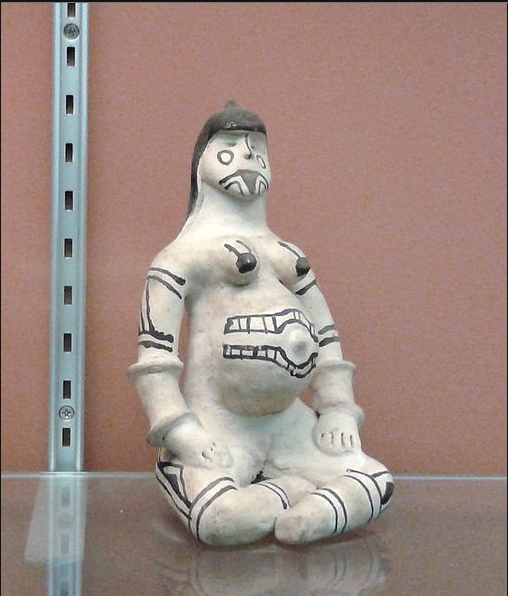
\includegraphics[width=4.00813in,height=4.70245in]{./imgSAEB_9_CHUM3/media/image1.png}
\caption{Uma imagem contendo edifício, foto, mesa, pintado Descrição
gerada automaticamente}
\end{figure}

a) Percebe-se que a pintura feita na boneca é igual àquela feita no
próprio corpo dos membros dessa população. O que explica tal fato?

Como cultura material do povo Karajá, a boneca expõe traços que
distinguem aquele povo como etnicamente diferenciados. As pinturas têm
significados cosmológicos para os Karajá, ou seja, fazem referência à
sua história mítica de criação. Os alunos podem se aproximar dessa
resposta se compreenderem que a pintura é uma forma de demonstrar a
diferenciação do povo.

\num{8} Leia os textos

\textbf{TEXTO 1}
\textbf{Geração nem-nem: jovens das favelas e periferias são menos favorecidosna hora de buscar oportunidades}

\begin{quote}
Você já ouviu falar na ``Geração nem-nem''? Esse termo é usado para se
referir aos jovens com idades entre 15 e 29 anos que estão fora do
mercado de trabalho e das instituições educacionais. De acordo com um
levantamento realizado pelo Centro de Políticas Sociais da Fundação
Getulio Vargas (FGV Social), no último trimestre de 2020, 25,5\% dos
jovens brasileiros se enquadram nessa situação. Embora muitos acreditem
que essa posição seja causada por falta de interesse e preguiça, a Tese
Social de Impacto em Empregabilidade feita pela Artemisia mostra que a
realidade é outra: a falta de oportunidades e de apoio é uma das
principais razões, especialmente para jovens de favelas e periferias.
\end{quote}

\fonte{de pesquisa: Janaína Dantas. Vozes das
periferias. Geração nem-nem: jovens das favelas e periferias são menos
favorecidosna hora de buscar oportunidades. Disponível em:
https://vozesdasperiferias.com/geracao-nem-nem-faltam-oportunidades-para-jovens.
Acesso em: 04 maio 2023.}

\textbf{TEXTO 2}
\textbf{PF mira grupo que alicia jovens no ES para levar drogas ao exterior}

A Justiça Federal de Vitória expediu cinco mandados de busca e
apreensão, que foram cumpridos pela Polícia Federal em dois locais do
Espírito Santo e três em Santa Catarina. Os investigados poderão
responder por tráfico internacional de drogas, associação para o tráfico
e, possivelmente, lavagem de dinheiro, com penas que podem chegar a 30
anos de prisão. Após a prisão de três pessoas em 2020, medidas de
cooperação internacional foram tomadas para obter provas que pudessem
ajudar a determinar os envolvidos no recrutamento de jovens no Espírito
Santo e no Brasil para atuar como ``mulas'' no tráfico internacional de
drogas.

\fonte{de pesquisa: Vinicius Zagoto. A Gazeta. PF mira
grupo que alicia jovens no ES para levar drogas ao exterior.
Disponível~em:~\textit{www.agazeta.com.br/es/policia/pf-mira-grupo-que-alicia-jovens-no-es-para-levar-drogas-ao-exterior-1022}.~Acesso~em:~07~mar.~2023.}

Estabeleça uma relação possível entre os dois textos. Apresente uma
introdução ao seu entendimento, desenvolva-o e conclua com sua opinião
sobre a relação entre os dois textos.

{A relação evidenciada é a de que jovens sem oportunidades tornam-se
vítimas do aliciamento criminoso. O aluno deve apresentar os fatos
retirados dos textos, relacioná-los e gerar uma conclusão opinativa a
partir disso, criando uma pequena
redação.\_\_\_\_\_\_\_\_\_\_\_\_\_\_\_\_\_\_\_\_\_\_\_\_\_\_\_\_\_\_\_\_\_\_\_\_\_\_\_\_\_\_\_\_\_\_\_\_\_\_\_\_\_\_\_\_\_\_\_\_\_\_\_\_\_\_\_\_\_\_\_\_\_\_\_\_\_\_\_\_\_\_\_\_\_\_\_\_\_\_\_\_\_\_\_\_\_\_\_\_\_\_\_\_\_\_\_\_\_\_\_\_\_\_\_\_\_\_\_\_\_\_\_\_\_\_\_\_\_\_\_\_\_\_\_\_\_\_\_\_\_\_\_\_\_\_\_\_\_\_\_\_\_\_\_\_\_\_\_\_\_\_\_\_\_\_\_\_\_\_\_\_\_\_\_\_\_\_\_\_\_\_\_\_\_\_\_\_\_\_\_\_\_\_\_\_\_\_\_\_\_\_\_\_\_\_\_\_\_\_\_\_\_\_\_\_\_\_\_\_\_\_\_\_\_\_\_\_\_\_\_\_\_\_\_\_\_\_\_\_\_\_\_\_\_\_\_\_\_\_\_\_\_\_\_\_\_\_\_\_\_\_\_\_\_\_\_\_\_\_\_\_\_\_\_\_\_\_\_\_\_\_\_\_\_\_\_\_\_\_\_\_\_\_\_\_\_\_\_\_\_\_\_\_\_\_\_\_\_\_\_\_\_\_\_\_\_\_\_\_\_\_\_\_\_\_\_\_\_\_\_\_\_\_\_\_\_\_\_\_\_\_\_\_\_\_\_\_\_\_\_\_\_\_\_\_\_\_\_\_\_\_\_\_\_\_\_\_\_\_\_\_\_\_\_\_\_\_\_\_\_\_\_\_\_\_\_\_\_\_\_\_\_\_\_\_\_\_\_\_\_\_\_\_\_\_\_\_\_\_\_\_\_\_\_\_\_\_\_\_\_\_\_\_\_\_\_\_\_\_\_\_\_\_\_\_\_\_\_\_\_\_\_\_\_\_\_\_\_\_\_\_\_\_\_\_\_\_\_\_\_\_\_\_\_\_\_\_\_\_\_\_\_\_\_\_\_\_\_\_\_\_\_\_\\
}

\section{Treino}

\num{1} Leia o texto.

\textbf{Unesco reconhece a capoeira como Patrimônio Cultural da Humanidade}

\begin{quote}
A Unesco declarou nesta quarta-feira (26) a capoeira como Patrimônio
Cultural Imaterial da Humanidade, reconhecendo-a como uma das
manifestações artísticas mais tradicionais do Brasil. Ao som do
berimbau, a capoeira mistura luta, dança e esporte, expressando a
cultura do povo brasileiro. Mestres brasileiros já difundiram a arte
para mais de 100 países, tornando-a um símbolo da cultura brasileira no
mundo todo. A presidente do Iphan, Jurema Machado, declarou estar
emocionada com o reconhecimento da capoeira como patrimônio mundial,
visto que ela foi criada por escravos e proibida por muitos anos no
Brasil.
\end{quote}

\fonte{de pesquisa: G1. Jornal Nacional, 26~nov.~2014.
Unesco reconhece a capoeira como Patrimônio Cultural da Humanidade.
Disponível~em:~\emph{https://g1.globo.com/jornal-nacional/noticia/2014/11/unesco-reconhece-capoeira-como-patrimonio-cultural-da-humanidade.html}.~Acesso~em:~07~mar.~2023.}

O reconhecimento da capoeira pela Unesco é importante por mostrar

\begin{enumerate}
\def\labelenumi{\alph{enumi})}
\item
  a importância da capoeira como expressão da humanidade.
\item
  a função da capoeira como luta de autodefesa feminina.
\item
  o papel da capoeira como patrimônio religioso.
\item
  o aspecto ambientalista da expressão.
\end{enumerate}

BNCC: EF09GE02 -- Analisar a atuação das corporações internacionais e
das organizações econômicas mundiais na vida da população em relação ao
consumo, à cultura e à mobilidade.

\begin{enumerate}
\def\labelenumi{\alph{enumi})}
\item
  Correta. Um patrimônio cultural imaterial corresponde a uma expressão
  representativa da diversidade sociocultural existente. Normalmente tem
  origem histórica longínqua e é praticado por grupos sociais coesos,
  como a população negra baiana, no caso da capoeira.
\item
  Incorreta. Apesar de poder ter essa função, não é o fator que gerou
  reconhecimento da capoeira como patrimônio imaterial.
\item
  Incorreta. Expressões religiosas podem ser reconhecidas como
  patrimônio cultural, porém a capoeira é uma expressão sem ligação
  obrigatória com a religião.
\item
  Incorreta. Trata-se de uma expressão sociocultural que, a princípio,
  não tem aspecto que a conecte a práticas ambientalistas.
\end{enumerate}

\num{2} Analise o esquema a seguir.

\begin{figure}
\centering
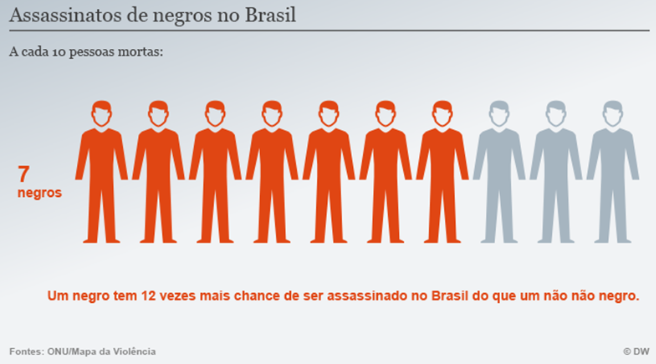
\includegraphics[width=5.90556in,height=3.27708in]{./imgSAEB_9_CHUM3/media/image2.png}
\caption{Texto Descrição gerada automaticamente}
\end{figure}

\textsubscript{.~Acesso~em:~08~de~mar.~2023.}

Identifica-se que a população negra é

\begin{enumerate}
\def\labelenumi{\alph{enumi})}
\item
  mais numerosa que a branca.
\item
  vítima preferencial da violência.
\item
  melhor posicionada economicamente.
\item
  mais escolarizada que a média nacional.
\end{enumerate}

BNCC: EF09HI26 -- Discutir e analisar as causas da violência contra
populações marginalizadas (negros, indígenas, mulheres, homossexuais,
camponeses, pobres etc.) com vistas à tomada de consciência e à
construção de uma cultura de paz, empatia e respeito às pessoas.

\begin{enumerate}
\def\labelenumi{\alph{enumi})}
\item
  Incorreta. O esquema trata da proporção, ou seja, das características
  apenas daqueles que foram vítimas de assassinato.
\item
  Correta. A proporção com maioria de negros mostra que essa população
  está inserida em contextos que a torna vítima preferencial de crimes
  de assassinato.
\item
  Incorreta. Inexiste qualquer informação no esquema que relacione o
  posicionamento econômico aos crimes de assassinato.
\item
  Incorreta. Inexiste qualquer informação sobre esse dado no esquema
  apresentado.
\end{enumerate}

\num{3} Considere os dados sobre mercado de trabalho a seguir.

\begin{figure}
\centering
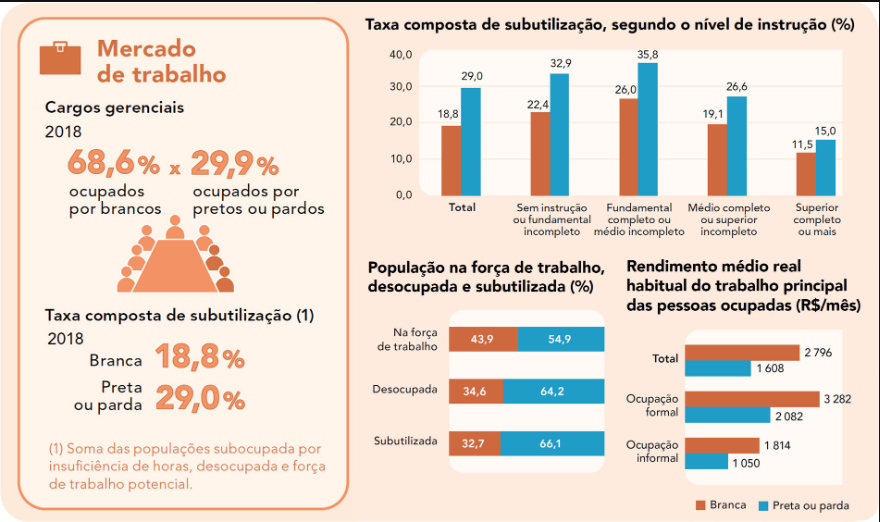
\includegraphics[width=5.27586in,height=3.12929in]{./imgSAEB_9_CHUM3/media/image3.png}
\caption{Interface gráfica do usuário, Aplicativo Descrição gerada
automaticamente}
\end{figure}

Qual das proposições a seguir é solução plausível para promover a
igualdade entre brancos e negros, considerando-se os dados apresentados?

\begin{enumerate}
\def\labelenumi{\alph{enumi})}
\item
  Criar mais vagas entre os cargos de menor remuneração.
\item
  Valorizar apenas o mérito como critério de promoção a cargos
  gerenciais.
\item
  Desenvolver a absorção e a qualificação profissional destinadas à
  população negra.
\item
  Validar o aumento da carga de trabalho da população negra
  economicamente ativa.
\end{enumerate}

BNCC: EF09HI26 -- Discutir e analisar as causas da violência contra
populações marginalizadas (negros, indígenas, mulheres, homossexuais,
camponeses, pobres etc.) com vistas à tomada de consciência e à
construção de uma cultura de paz, empatia e respeito às pessoas.

\begin{enumerate}
\def\labelenumi{\alph{enumi})}
\item
  Incorreta. Tal proposta não resolve dois dos problemas apresentados,
  que são a baixa ocupação de cargos gerenciais por pessoas negras e o
  menor rendimento médio dessa população.
\item
  Incorreta. A alternativa não é viável, pois o baixo número de pessoas
  negras em cargos mais elevados não permitiria que apenas o mérito
  promovesse uma maior integração econômica e profissional dessa
  população.
\item
  Correta. Tal alternativa tem potencial de atacar todos os problemas
  apresentados, pois a maior qualificação profissional ampliaria as
  oportunidades para essa população, que também seria beneficiada por
  programas de reserva de vagas em cargos mais elevados, o que
  contribuiria também para o aumento do rendimento médio e a melhor
  utilização do potencial profissional dessa população.
\item
  Incorreta. Tal alternativa não ataca nenhum dos problemas
  apresentados, além de ser potencialmente danosa à população negra, que
  já enfrenta grandes dificuldades para a composição do orçamento
  doméstico.
\end{enumerate}

\chapter{O Estado}
\markboth{Módulo 4}{}

\section{Eixo de conhecimento do SAEB} Poder, estado e instituições.

<<<<<<< HEAD
\section{Habilidade da BNCC} EF09GE08
=======
\subsection{Habilidade da BNCC} EF09GE08
>>>>>>> 92e3cd6407615258ebd886843e38a91cbf55d87c

\conteudo{Poder, estado e instituições são conceitos inter-relacionados que descrevem as complexas dinâmicas do sistema político em uma sociedade. O poder pode ser definido como a capacidade de influenciar e controlar as decisões e ações de outros indivíduos ou grupos. O estado, por sua vez, é uma estrutura política que detém o poder soberano sobre uma determinada área geográfica, com autoridade para impor leis e regulamentos, cobrar impostos e administrar a justiça. As instituições, por fim, são os órgãos e mecanismos formais que permitem que o estado exerça seu poder, como o legislativo, o executivo e o judiciário.

A relação entre esses três conceitos é complexa e pode variar de acordo com o tipo de estado e a sua história política. Em geral, as instituições são criadas pelo estado para exercer seu poder de forma organizada e institucionalizada. Elas são responsáveis por regulamentar a vida política, social e econômica de uma sociedade e garantir o cumprimento das leis e das normas.

O poder, por sua vez, pode ser exercido dentro ou fora dessas instituições, tanto pelo estado quanto por atores políticos externos. As relações de poder podem ser simétricas ou assimétricas, dependendo da capacidade de cada ator político de influenciar ou controlar as decisões e ações dos outros. A capacidade de exercer o poder pode ser influenciada por vários fatores, como a riqueza, a posição social, a educação, a habilidade política e a força militar.

As instituições do estado podem ser vistas como um meio de equilibrar as relações de poder, estabelecendo regras claras e garantindo a participação cidadã nas decisões políticas. No entanto, as instituições também podem ser usadas como mecanismos de controle e dominação por parte dos grupos dominantes, reforçando as desigualdades sociais e econômicas. Portanto, a relação entre poder, estado e instituições é dinâmica e exige uma análise crítica constante para entender e promover a justiça e a igualdade na sociedade.}

\section{Atividades}

Leia o texto para resolver as atividades 1 e 2.

\textbf{Projeto S é exemplo de como incentivar a vacinação e combater a desinformação}

\begin{quote}
{[}\ldots{}{]}

Mesmo em um cenário de negacionismo e de grande disseminação de notícias
falsas sobre vacinas, o Projeto S --- estudo de efetividade da vacina
Coronavac na cidade de Serrana/SP --- teve sucesso em aumentar a
credibilidade da CoronaVac ao apresentar dados do mundo real que
comprovam a sua efetividade.
\end{quote}

\begin{quote}
``A estreita coordenação entre pesquisadores, autoridades locais e
estaduais e líderes comunitários foi fundamental para tornar este estudo
possível e se refletiu na alta aceitação da vacina. O papel dos líderes
comunitários na promoção do programa de vacinação do estudo também foi
um aspecto essencial para o sucesso da imunização'', destacam os
pesquisadores no artigo sobre o Projeto S, que foi~publicado e
encaminhado à revista científica \emph{Lancet} {[}\ldots{}{]}.
\end{quote}

\begin{quote}
{[}\ldots{}{]}
\end{quote}

\fonte{Portal do Butantan. Projeto S é exemplo de como
incentivar a vacinação e combater a desinformação. Disponível em:
https://butantan.gov.br/noticias/projeto-s-e-exemplo-de-como-incentivar-a-vacinacao-e-combater-a-desinformacao.
Acesso em: 07 mar. 2023.}

\num{1} O Brasil tem um histórico positivo em relação às campanhas de
vacinação contra diversos agentes infecciosos. Mesmo assim, durante a
pandemia de covid-19, foi necessário grande esforço para levar a
população aos locais de aplicação das vacinas, inclusive por parte de
agentes não estatais. Tendo em vista o trecho publicado, qual foi a
importância dos líderes comunitários para o sucesso da campanha de
vacinação?

\reduline{Os líderes comunitários têm grande permeabilidade e influência dentro
dos limites territoriais em que atuam, tendo sido um importante veículo
de propagação e esclarecimento da campanha de vacinação.}

\num{2} A figura do Estado foi vital para o controle e o enfrentamento
da pandemia de covid-19, contudo outros agentes também foram essenciais
e nortearam as ações estatais ao longo da pandemia. Além dos líderes
comunitários, quem são os agentes que auxiliaram o Estado nesse
enfrentamento?

\reduline{Foram os pesquisadores e os médicos, além das autoridades públicas.}

\num{3} Leia o texto.

\begin{quote}
Mais de um quarto dos bairros do Rio de Janeiro (25,5\%) estão sob o
controle das milícias, abrangendo 57,5\% do território da cidade. As
três principais facções criminosas envolvidas no tráfico de drogas -
Comando Vermelho, Terceiro Comando e Amigos dos Amigos - controlam
juntas 34,2\% dos bairros e 15,4\% do território. Isso significa que
cerca de 3,7 milhões de pessoas vivem em áreas dominadas por grupos
criminosos, o que equivale a 57,1\% da população da cidade.
\end{quote}

\fonte{de pesquisa: Aiuri Rebello. El País. Milícias já
dominam um quarto dos bairros do Rio de Janeiro, com quase 60\% do
território da cidade.
Disponível~em:~https://brasil.elpais.com/brasil/2020-10-19/milicias-ja-dominam-um-quarto-dos-bairros-do-rio-de-janeiro-com-quase-60-do-territorio-da-cidade.html.~Acesso~em:~03~mar.~2023.}

O fortalecimento de grupos criminosos tem sido uma constante nas últimas
décadas no Brasil, mais especificamente no estado do Rio de Janeiro. A
milícia e o tráfico controlam territórios e diversos tipos de serviço,
públicos e privados. Tendo em vista essa expansão, cite um motivo que
justifique o crescimento do domínio desses grupos.

\reduline{O crescimento de tais grupos foi resultado do fracasso de políticas
públicas, especificamente do setor de segurança. O Estado tem sido
ineficiente em combater as ações desses grupos, além de conter sua
expansão.}

\num{4} Leia o texto.

\textbf{Vaias ao hino espanhol na final da Copa do Rei rendem multa de 246 mil ao Barcelona}

\begin{quote}
A Comissão antiviolência da federação espanhola anunciou as punições
decorrentes das vaias ao hino espanhol durante a final da Copa do Rei
entre Barcelona e Athletic Bilbao. O clube catalão, campeão do torneio,
recebeu a multa mais pesada dos dois finalistas, no valor de 60 mil
euros (cerca de R\$ 246 mil). Já o Bilbao, vice-campeão, foi multado em
18 mil euros (cerca de R\$ 67 mil). Embora as vaias tenham partido da
torcida catalã, a comissão antiviolência decidiu punir o clube por
omissão às ameaças de vaia, que já eram previamente conhecidas.
\end{quote}

\fonte{de pesquisa: Extra. Vaias ao hino espanhol na
final da Copa do Rei rendem multa de R\$ 246 mil ao Barcelona.
Disponível~em:~https://extra.globo.com/esporte/vaias-ao-hino-espanhol-na-final-da-copa-do-rei-rendem-multa-de-246-mil-ao-barcelona-16981835.html.~Acesso~em:~03~mar.~2023.}

A população da Catalunha e dos Países Bascos, sedes dos clubes Barcelona
e Athletic Bilbao, respectivamente, reconhecem-se enquanto espanhóis.

Você concorda com essa afirmativa ou discorda dela? Justifique.

\reduline{O aluno deve discordar. Catalães e bascos não se reconhecem enquanto espanhóis, dada a
anexação forçada das duas regiões pelo Estado espanhol no passado.
Além disso, durante o século XX, foram povos que sofreram com a ditadura
franquista --- inclusive a população foi cerceada das culturas e das línguas
locais ---, o que fomentou um sentimento de repulsa ao Estado espanhol. Por
isso, ocorreram as vaias ao hino nacional na partida citada. Ademais, recentemente,
a população da Catalunha votou em favor de um referendo que pede a
independência da região frente à Espanha.}

\num{5} Espalhados pelos territórios de cinco países (Turquia, Iraque,
Síria, Irã e Armênia), os curdos totalizam algo entre 25 e 35 milhões de
pessoas. Apesar de formarem o quarto maior grupo étnico do Oriente
Médio, nunca conseguiram um país próprio. Independentemente da origem,
os curdos compõem um grupo populacional numeroso e têm como objetivo a
formação de um Estado. Explique a dificuldade dos curdos de conseguirem
o objetivo de formação de um Estado próprio.

\reduline{Os curdos podem ser entendidos enquanto nação, ou seja, um grupo com
similaridades étnicas e objetivos em comum; contudo a formação do
Estado curdo é dificultada pela ausência de território, uma vez que os
locais onde os curdos vivem atualmente abrigam Estados nacionais já
formados e reconhecidos internacionalmente. Dessa forma, a obtenção de
um território para a formação do Curdistão compreende um assunto muito
delicado, que envolve outros Estados nacionais.}

\num{6} A maioria separatista do Parlamento catalão proclamou
unilateralmente a independência da Catalunha, encerrando quase um mês de
incerteza após o referendo de autodeterminação ocorrido em 1º de
outubro, apesar da suspensão da Justiça espanhola. Como esperado, no
entanto, as instituições europeias e os países do bloco, como França,
Alemanha e Reino Unido, não reconheceram a declaração. Em Berlim, um
porta-voz afirmou que a soberania e a integridade territorial da Espanha
são e continuarão sendo invioláveis. Mesmo sendo desejo de maioria da
população da Catalunha, o processo de independência da região está longe
de ser realidade. Qual é o entrave à obtenção da independência catalã?

\reduline{O entrave é o não reconhecimento de órgãos
internacionais, como a União Europeia. Para a formação de um novo
Estado nacional, é vital obter o reconhecimento internacional, seja de
países, seja de instituições, seja de blocos.}

\num{7} De 1917 até a atualidade, o mundo acompanha a evolução do
território israelense e a redução do território ocupado pelos
palestinos. Aponte e explique a razão dos conflitos entre israelenses e
palestinos.

\reduline{A razão para os conflitos entre judeus e palestinos a partir da criação
do Estado de Israel (1947) é o avanço territorial dos israelenses,
incorporando áreas antes controladas pelos árabes. Além disso, os
palestinos reivindicam a criação de um Estado próprio, no mesmo
território onde está situado o Estado israelense, o que complica uma
resolução de paz para esses povos.}

\num{8} Atribua V (verdadeiro) e F (falso) para as afirmativas a seguir.

(V) A existência de um Estado demanda, necessariamente, um território.

(F) Os palestinos e os curdos lutam pela formação de suas respectivas
nações.

(V) A formação de um novo Estado nacional demanda a realização de
consulta popular.

(V) Os pedidos de independência estão ligados à falta de pertencimento à
unidade territorial central.

\num{9} Ao longo do processo de formação dos Estados, diversas
comunidades foram reunidas em um mesmo território, submetidas a um mesmo
governo e às mesmas leis, independentemente de sua origem ou tamanho.
Como resultado das guerras de conquista, povos menores foram agrupados
com os maiores. Por outro lado, o nacionalismo é um movimento que se
baseia no sentimento de lealdade à nação por parte de um grupo de
pessoas que compartilham tradições, língua, cultura, religião ou
interesses comuns e que busca estabelecer uma identidade política
autônoma e o direito à autodeterminação. Nem sempre, porém, o
nacionalismo é reconhecido pelas autoridades governamentais, que podem
manter a soberania e a integridade territorial do Estado em detrimento
das reivindicações nacionalistas. Que povos estão inseridos nesse
contexto?

\reduline{Estão inseridos nesse contexto: curdos, catalães, bascos e palestinos.}

\num{10} De um lado, gritos de ``Barcelona, vocês sempre serão
Espanha!''. De outro, faixas da torcida do Barcelona pedindo liberdade.
Esse era o cenário de um jogo pelas oitavas de final da Liga dos
Campeões no estádio Camp Nou, em Barcelona. Qual é o motivo para a
veiculação da mensagem sobre liberdade em jogos internacionais do
Barcelona?

\reduline{Devido à globalização, os jogos de futebol têm uma abrangência muito
grande, fazendo com que a mensagem de protesto seja ecoada em muitos
lugares. Nesse caso, a Catalunha deseja ser uma região independente da
Espanha, mas carece também de reconhecimento internacional para a
formação de um novo Estado. Por isso, é importante que ocorra a
manifestação dos locais, na tentativa de tentar transmitir o sentimento
nacional, divergente da unidade territorial espanhola.}

\section{Treino}

\num{1} Leia o texto.

\textbf{Independência da Catalunha vence referendo com 90\% dos votos, diz governo catalão}

\begin{quote}
Na noite deste domingo (1º), o presidente da Catalunha, Carles
Puigdemont, declarou que o referendo sobre a independência da região da
Espanha concedeu à Catalunha o ``direito de ser um Estado''. Segundo
ele, os cidadãos catalães conquistaram ``o direito de ter um estado
independente na forma de uma república'' e ``o direito de serem ouvidos,
respeitados e reconhecidos''. O referendo resultou em uma vitória
esmagadora do ``Sim'', com 90,09\% dos votos (2.020.144 votos), enquanto
o ``Não'' obteve 7,87\% (176.565 votos). Os votos em branco foram 2,03\%
(45.586); os nulos, 0,89\% (20.129). De acordo com o governo catalão,
foram registrados um total de 2.262.424 votos.
\end{quote}

\fonte{de pesquisa: G1. Independência da Catalunha vence
referendo com 90\% dos votos, diz governo catalão. Disponível em:
https://g1.globo.com/mundo/noticia/presidente-catalao-diz-que-catalunha-ganhou-direito-de-ser-um-estado-premie-espanhol-afirma-que-nao-houve-referendo.ghtml.
Acesso em: 08 mar. 2023.}

Tendo em vista a aprovação do referendo, conclui-se que os catalães
demonstraram

\begin{enumerate}
\def\labelenumi{\alph{enumi})}
\item
  sua territorialidade.
\item
  sua nacionalidade.
\item
  seu apartidarismo.
\item
  sua legitimidade.
\end{enumerate}

BNCC: EF09GE08 -- Analisar transformações territoriais, considerando o
movimento de fronteiras, tensões, conflitos e múltiplas regionalidades
na Europa, na Ásia e na Oceania.

a) Correta. Ao aprovar o referendo em prol da independência da região,
os catalães demonstram sua territorialidade, ou seja, seu sentimento de
pertencimento à Catalunha, e não ao Estado espanhol.

b) Incorreta. A nação catalã, ou seja, o grupo de pessoas com traços
étnicos e culturais em comum, existe independentemente do referendo.

c) Incorreta. O referendo compreende a consulta popular sobre
determinado tema, mas que não envolve a escolha por partidos políticos
ou o seu rechaço em relação a eles.

d) Incorreta. O referendo é uma das etapas dos catalães em busca de sua
legitimidade frente ao Estado espanhol, ou seja, a conquista de sua
independência. Sua realização e aprovação não resultou, diretamente, na
independência da Catalunha, tanto é que não foi considerado legítimo
pelo governo espanhol.

\num{2} Leia o texto.

\textbf{Ministério da Saúde anuncia um dos embaixadores da Campanha Nacional de Vacinação}

\begin{quote}
O Ministério da Saúde anunciou, nesta quarta-feira (08), um dos
embaixadores da Campanha Nacional de Vacinação deste ano. O influencer
Ivan Baron, do Rio Grande do Norte, é ativista pela causa das pessoas
com deficiência {[}\ldots{}{]}.
\end{quote}

\begin{quote}
Ivan Baron falou sobre a importância da vacinação das pessoas com
deficiência e a relevância das políticas públicas inclusivas. ``Todos
nós temos esse compromisso com a saúde pública {[}\ldots{}{]}.''
\end{quote}

\begin{quote}
{[}\ldots{}{]}
\end{quote}

\fonte{Ministério da Saúde. Ministério da Saúde anuncia um dos
embaixadores da Campanha Nacional de Vacinação.
Disponível~em:~https://www.gov.br/saude/pt-br/assuntos/noticias/2023/fevereiro/ministerio-da-saude-anuncia-embaixador-da-campanha-nacional-de-vacinacao.~Acesso~em:~03~mar.~2023.}

A escolha de um \emph{digital influencer} para estimular campanhas
públicas de vacinação explica-se

\begin{enumerate}
\def\labelenumi{\alph{enumi})}
\item
  pelo descontentamento da população com os resultados de testes das
  vacinas.
\item
  pelo reconhecimento dos \emph{influencers} pelo público geral.
\item
  pela repulsa populacional às campanhas públicas de vacinação.
\item
  pelo rechaço da população às figuras políticas e públicas.
\end{enumerate}

a) Incorreta. A importância de se vacinar é reforçada nas campanhas de
vacinação, além do fato de não se escolher os imunizantes
disponibilizados. Nesse caso, a escolha dos \emph{influencers} não visa
remediar descontentamento com resultados de testes.

b) Correta. \emph{Influencers} são reconhecidos pela sociedade, ou por
grupos mais específicos, e suas ações muitas vezes servem como estímulos
para pessoas não famosas.

c) Incorreta. O texto não destaca a repulsa da população pelas campanhas
vacinais.

d) Incorreta. O texto não destaca o rechaço da população às figuras
públicas.

\num{3} Leia o texto.

\textbf{Tráfico e milícia já controlam 80\% da venda de botijões de gás no estado do Rio}

\begin{quote}
Alexandre José Borjaili, presidente da Associação Brasileira dos
Revendedores de GLP (Asmirg) há 15 anos, lamenta a situação do mercado
de gás no Rio de Janeiro, que se tornou uma realidade à parte no setor.
Mesmo com revendas regularizadas, funcionários correm risco de morte ao
fazer negócios fora do estabelecimento. Segundo ele, de 70\% a 80\% do
mercado do estado está nas mãos do crime organizado, tornando difícil
para qualquer ação do governo chegar ao consumidor final. Borjaili
ressalta que essa realidade não se aplica apenas ao vale-gás, mas também
quando há controle de preços por políticas estatais. Se o crime controla
a venda, qualquer ação governamental acaba sendo inútil.
\end{quote}

\fonte{de pesquisa: Luã Marinatto. Extra. Tráfico e
milícia já controlam 80\% da venda de botijões de gás no estado do Rio.
Disponível~em:~https://extra.globo.com/casos-de-policia/trafico-milicia-ja-controlam-80-da-venda-de-botijoes-de-gas-no-estado-do-rio-25365008.html.~Acesso~em:
03~mar.~2023.}

A situação descrita no texto exemplifica

\begin{enumerate}
\def\labelenumi{\alph{enumi})}
\item
  a transferência do monopólio da força do Estado para o crime
  organizado.
\item
  o reconhecimento da legitimidade do crime organizado pelo Estado.
\item
  a aceitação da população frente às atividades do crime organizado.
\item
  a regulação da atividade comercial pelo crime organizado.
\end{enumerate}

a) Incorreta. O Estado brasileiro não está transferindo o monopólio da
força para as mãos do crime organizado.

b) Incorreta. Na situação descrita, não há reconhecimento da
legitimidade do crime organizado pelo Estado. No caso, houve a imposição
da força pelo crime organizado, que resultou no domínio das atividades
comerciais.

c) Incorreta. O texto não destaca a aceitação populacional das ações do
crime organizado. Na realidade, o cumprimento das imposições feitas
pelos criminosos se dá para a manutenção da segurança e da integridade
próprias.

d) Correta. O texto destaca que o crime organizado controla o mercado de
gás em áreas de comunidade, impondo seus preços e locais de compra, à
revelia das determinações do Estado e de sua regulação de preços. A
``obediência'' às regras impostas pelo crime organizado é explicada pela
manutenção da segurança e da integridade dos populares.

\chapter{Direitos humanos}
\markboth{Módulo 5}{}

\section{Eixo de conhecimento do SAEB} Cidadania, direitos humanos e
movimentos sociais.

<<<<<<< HEAD
\section{Habilidades da BNCC} EF09HI07, EF09HI09, EF09HI16, EF09HI21,
=======
\subsection{Habilidades da BNCC} EF09HI07, EF09HI09, EF09HI16, EF09HI21,
>>>>>>> 92e3cd6407615258ebd886843e38a91cbf55d87c
EF09HI23.

\conteudo{Os direitos humanos são um conjunto de normas e princípios que garantem a dignidade, liberdade e igualdade de todos os seres humanos, independentemente de sua origem, raça, religião, gênero, orientação sexual ou qualquer outra condição.

Esses direitos são fundamentais para a construção de uma sociedade justa e democrática, onde todas as pessoas possam desfrutar de oportunidades iguais e viver com segurança e respeito. Eles são protegidos por leis internacionais e nacionais, e devem ser respeitados por governos, empresas e indivíduos.

Entre os direitos humanos mais importantes estão o direito à vida, à liberdade e à segurança pessoal, à igualdade perante a lei, à liberdade de pensamento, expressão e religião, ao trabalho digno, à educação e à saúde. A proteção desses direitos é essencial para o bem-estar das pessoas e para o desenvolvimento sustentável de todas as nações.}

Leia os textos para resolver as atividades 1 e 2.

\textbf{TEXTO 1}
\textgreater{}\textbf{Serviço de Proteção aos Índios e Localização dos Trabalhadores Nacionais}

\begin{quote}
O Serviço de Proteção aos Índios e Localização dos Trabalhadores
Nacionais foi criado pelo decreto n. 8.072, de 20 de junho de 1910, com
a finalidade de prestar assistência aos~indígenas do Brasil e
estabelecer centros agrícolas, constituídos pelos chamados trabalhadores
nacionais.
\end{quote}

\begin{quote}
A incorporação dos indígenas~e dos trabalhadores nacionais no processo
produtivo e o combate ao êxodo rural figuraram na pauta dos debates
realizados pelos representantes dos setores agrícolas distanciados do
centro de poder, que estiveram na origem da criação do~Ministério da
Agricultura, Indústria e Comércio~em 1906. Se nas áreas de plantio de
café, a mão de obra era suprida pelos imigrantes, nas outras regiões se
faziam necessárias medidas voltadas para os ``nacionais'', denominação
que abrangia ex-escravizados e seus descendentes, sertanejos e outros
grupos (Mendonça, 1997, p.~85; 168). Assim, promover uma melhor
distribuição espacial da força de trabalho e administrar os conflitos
indígenas resultantes, especialmente, do processo de especulação de
terra impulsionado pela expansão da rede ferroviária, constituíram-se
como objetivos da ação do Estado por meio do Serviço de Proteção aos
Índios e Localização dos Trabalhadores Nacionais, de forma a contribuir
para ``o alargamento das fronteiras, simbólicas e econômicas, da
Nação{]}\{.underline\}'' (Mendonça, 1997, p.~168).
\end{quote}

\begin{quote}
{[}...{]}
\end{quote}

\fonte{Memória da Administração Pública Brasileira. Serviço de
Proteção aos Índios e Localização dos Trabalhadores Nacionais.
Disponível em:
http://mapa.an.gov.br/index.php/ultimas-noticias/686-servico-de-protecao-aos-indios-e-localizacao-dos-trabalhadores-nacionais.
Acesso em: 09 mar. 2023.}

\textbf{TEXTO 2} \textgreater{}\textbf{Os Xokleng}

\begin{quote}
Os Xokleng, povo indígena da Terra Indígena Ibirama em Santa Catarina,
são sobreviventes de um processo brutal de colonização do sul do Brasil,
iniciado no século passado, que quase os levou à extinção. Embora alguns
subgrupos Xokleng tenham sido exterminados no estado e os sobreviventes
confinados em uma área delimitada em 1914, para garantir a ``paz'' aos
colonos e a expansão do vale do rio Itajaí, os Xokleng persistem em
lutar pela sobrevivência diante desta invasão, mesmo após a quase
extinção dos recursos naturais de sua terra, agravada pela construção da
Barragem Norte.
\end{quote}

\fonte{de pesquisa: Povos Indígenas do Brasil. Xokleng.
Disponpível em: https://pib.socioambiental.org/pt/Povo:Xokleng. Acesso
em: 09 mar. 2023.}

\num{1} Com base nos textos, como podemos caracterizar a relação da
sociedade brasileira com as populações indígenas no começo do século XX?

\reduline{No primeiro texto, fica claro o papel do Estado como apaziguador dos
conflitos entre o avanço de atividades econômicas capitalistas e as
populações indígenas. Já no segundo texto, a menção à diminuição dos recursos
naturais mostra que existia uma disputa pelo acesso aos recursos, sendo
utilizado inclusive o confinamento de populações indígenas para melhor
espoliação dos recursos naturais.}

\num{2} No texto 2, está implícita a principal causa dos conflitos entre
população indígena e não indígena no período. Qual seria essa causa?

\reduline{Trata-se da disputa pela posse do território e dos recursos naturais existentes.}

\num{3} Leia os textos.

\textbf{TEXTO 1}
\textgreater{}\textbf{A rodovia transamazônica e os indígenas tenharim: ontem e hoje}

\begin{quote}
Manoel Duca, cacique da aldeia Bela Vista, de 52 anos, relatou em um
depoimento que os indígenas Tenharim tinham muito medo dos trabalhadores
da rodovia Transamazônica. Segundo ele, apenas três indígenas
representavam o povo, enquanto os outros se escondiam no mato. A empresa
responsável pela construção contratou os indígenas para fazer a
desmatação, usando como incentivo o machado e a promessa de abrir a
estrada. Durante um ano, trabalharam sem receber salário até a
localidade Matamata, à margem do rio Aripuanã, derrubando árvores,
inclusive dentro d'água. Os empregados das empreiteiras ordenavam aos
indígenas nas aldeias: ``Sai da frente!''. A alimentação era
insuficiente e a cultura dos indígenas foi perdida, incluindo as frutas
encontradas no traçado da estrada e as redes de algodão que eles
próprios faziam. Manoel Duca destacou que eles eram tratados como
prisioneiros e eram obrigados a obedecer às ordens dos seus
empregadores.
\end{quote}

\fonte{de pesquisa: Julio José Araújo Junior. ANPR.
Disponível~em:~https://www.anpr.org.br/imprensa/artigos/20875-a-rodovia-transamazonica-e-os-indigenas-tenharim-ontem-e-hoje.~Acesso~em:
10~mar.~2023.}

\textbf{TEXTO 2}
\textgreater{}\textbf{Indígenas Tenharim pedem regularização das barreiras na Br 230/ Transamazônica e denunciam retirada ilegal de madeira e existência de assentamento do Incra dentro de Terra Indígena}

\begin{quote}
A Organização dos Povos Indígenas do Alto Madeira (OPIAM) e a
Coordenação das Organizações Indígenas da Amazônia Brasileira (Coiab)
protocolaram, em 17/01, documentos no Ibama e Incra, denunciando a
retirada ilegal de madeira e a presença de assentamentos do Incra dentro
das Terras Indígenas Tenharim do Marmelo/Gleba B e Sepoti, localizadas
nos municípios de Manicoré e Humaitá, no sul do Amazonas. Os Tenharim
também entregaram documentos na Procuradoria da República no Amazonas,
denunciando a instalação de barreiras na BR 230/Transamazônica dentro
das terras indígenas e pedindo indenização e regularização das mesmas.
Juntamente com os documentos, eles apresentaram ao Ministério Público
Federal um relatório de estudo de impacto ambiental, cultural e
antropológico realizado nas proximidades da BR. Os indígenas solicitaram
ação das autoridades competentes para solucionar a situação.
\end{quote}

\fonte{de pesquisa: Coiab. Instituto Socioambienta.
Indígenas Tenharim pedem regularização das barreiras na Br 230/
Transamazônica e denunciam retirada ilegal de madeira e existência de
assentamento do Incra dentro de Terra Indígena.
Disponível~em:~https://acervo.socioambiental.org/acervo/noticias/indigenas-tenharim-pedem-regularizacao-das-barreiras-na-br-230-transamazonica-e.~Acesso~em:~10~mar.~2023.}

Os textos fazem menção a momentos distintos para uma mesma área. No
primeiro, fala-se sobre o processo de abertura da rodovia federal BR-230
nos anos de 1970, mais conhecida como Transamazônica, enquanto, no
segundo texto, fala-se sobre sua utilização nos dias de hoje. A partir
da leitura dos textos, identifique os impactos da criação da rodovia
Transamazônica para os indígenas locais.

\reduline{A implantação da rodovia Transamazônica foi uma das razões de
aproximação entre indígenas e os demais grupos étnicos na região Norte, que passaram a ocupá-la e desenvolvê-la em prol do dinamismo
e do crescimento econômico local. Essa aproximação, contudo, foi muito
sentida pelos indígenas, uma vez que o contato com outros povos fez com
que estivessem sujeitos a crimes, como o trabalho análogo à escravidão, e doenças trazidas de fora, além da destruição dos
recursos naturais locais. A manutenção da Rodovia e das atividades
predatórias fez com que os indígenas se organizassem, criando
instituições capazes de denunciar as irregularidades que ocorrem em seus
territórios. É importante frisar que a lógica imposta pelo capital sobre o território é distinta da lógica imposta pelos indígenas, que pautam a
subsistência.}

\num{4} Leia o texto.

\begin{quote}
\textbf{Ocupações em São Paulo}
\end{quote}

\begin{quote}
``Realizamos uma assembleia ontem, mas não chegamos a uma conclusão.
Hoje à noite, teremos outra para decidir se vamos ocupar ou não a
escola.'', disse Douglas, de 17 anos, aluno do terceiro ano da Escola
Estadual Diadema. O discurso dele parece uma repetição do passado. Há um
ano, antes da escola ser a primeira a ser ocupada no Estado de São Paulo
em protesto contra a reorganização escolar proposta pelo Governo Alckmin
(PSDB), ele poderia ter dito exatamente a mesma coisa. Mas, na verdade,
ele falou isso na semana passada, em frente à escola. Douglas mencionou
a possibilidade de repetir um movimento que cresceu no final de 2015,
culminando na derrubada do então secretário de Educação do Estado de São
Paulo e na suspensão, pelo menos temporária, do projeto que fecharia 92
escolas.

Douglas foi um dos principais envolvidos na ocupação da E. E. Diadema em
9 de novembro do ano passado. Naquela época, ninguém poderia imaginar
que isso seria o início de um movimento em cascata que rapidamente se
espalharia para mais de 200 escolas ocupadas em todo o Estado. As
ocupações foram a segunda fase de uma luta iniciada com
abaixo-assinados, protestos nas ruas e tentativas, sem sucesso, de
conversas com os dirigentes de ensino.

Naquela época, os alunos exigiam mais explicações sobre o projeto que
foi anunciado às pressas. O Governo alegava que as escolas de ciclos
únicos --- aquelas que oferecem apenas o Ensino Médio ou apenas o Ensino
Fundamental --- apresentavam melhores resultados acadêmicos. Além disso,
argumentava que o número de salas ociosas havia aumentado nos últimos
anos e era necessário um remanejamento para otimizar os espaços.
\end{quote}

\fonte{de pesquisa: Marina Rossi. El País. Reforma do
Ensino Médio reacende mobilização um ano após ocupações em São Paulo.
Disponível em:
https://brasil.elpais.com/brasil/2016/10/14/politica/1476476414\_549165.html.
Acesso em: 10 mar. 2023.}

A reorganização escolar de 2015 foi uma tentativa de reorganização das
escolas do estado de São Paulo por meio da centralização das matrículas
disponíveis em menos escolas. De acordo com o texto, explique dois fatos
que levaram à não aplicação dessa reforma.

\reduline{A reforma, conhecida como "reorganização escolar", não foi efetivada em
razão dos protestos promovidos pelos estudantes, além das decisões
judiciais que a contestaram.}

\num{5} Martin Luther King (1929-1968) notabilizou-se por sua liderança
aos protestos não violentos e ao movimento pelos direitos sociais e
civis dos negros nos Estados Unidos da América. O trecho a seguir faz
parte do discurso proferido pelo reverendo King, após a decisão da
Suprema Corte dos Estados Unidos tornar ilegal a segregação nos ônibus
na cidade de Montgomery, em 1956.

\begin{quote}
Este é um momento em que devemos agir com dignidade e prudência. Não
devemos permitir que nossas emoções nos dominem ou que a violência nos
defina. Se formos alvos de atos violentos, todo o nosso esforço para
alcançar uma vida digna terá sido em vão, e nossos doze meses de luta
gloriosa serão vistos como um prelúdio para uma catástrofe sombria.
Enquanto voltamos para os ônibus, devemos ser suficientemente amorosos
para transformar nossos inimigos em amigos. É hora de mudarmos nossa
abordagem do protesto para a conciliação.
\end{quote}

A partir do trecho, analise a importância de ações não violentas nos
protestos organizados por King a fim de conquistar a dessegregação nos
ônibus em Montgomery.

\reduline{Martin Luther King buscava chamar a atenção dos negros e das autoridades
públicas --- políticos e líderes de organização --- para a injustiça sofrida
por seus semelhantes, além de que a prática de protesto não violento
atenuava a agressividade imposta pelos agentes do Estado.}

\num{6} Leia os textos de dois artigos da ``Declaração universal dos
direitos humanos''.

\begin{quote}
\textbf{Artigo 3} Todo ser humano tem direito à vida, à liberdade e à
segurança pessoal.
\end{quote}

\begin{quote}
\textbf{Artigo 4} Ninguém será mantido em escravidão ou servidão; a
escravidão e o tráfico de escravos serão proibidos em todas as suas
formas.
\end{quote}

Após a leitura dos artigos, analise a notícia reproduzida a seguir.

\begin{quote}
\textbf{Vinícolas devem pagar R\$ 7 milhões por caso de trabalho escravo no RS}
\emph{Uma parte é por danos morais coletivos e outra, individuais}
\end{quote}

\begin{quote}
{[}\ldots{}{]}
\end{quote}

\begin{quote}
Em 22 de fevereiro {[}de 2023{]}, uma ação conjunta entre a Polícia
Rodoviária Federal (PRF), Polícia Federal (PF) e Ministério do Trabalho
e Emprego (MTE) resgatou 207 trabalhadores que enfrentavam condições de
trabalho degradantes em Bento Gonçalves, na Serra Gaúcha.
\end{quote}

\begin{quote}
O resgate ocorreu depois que três trabalhadores que fugiram do local
contactaram a PRF, em Caxias do Sul (RS), e fizeram a denúncia.
\end{quote}

\begin{quote}
Atraídos pela promessa de salário de R\$ 3 mil, os trabalhadores
relataram enfrentar atrasos nos pagamentos dos salários, violência
física, longas jornadas e oferta de alimentos estragados.
\end{quote}

\begin{quote}
Eles relataram ainda que, desde que chegaram, no início do mês, eram
coagidos a permanecer no alojamento, sob pena de pagar multa por quebra
do contrato de trabalho. A PF prendeu um empresário baiano responsável
pela empresa, que foi encaminhado para o presídio de Bento Gonçalves.
\end{quote}

\begin{quote}
Em notas, as vinícolas envolvidas disseram que desconheciam as
irregularidades praticadas contra os trabalhadores recrutados pela
empresa prestadora de serviços terceirizados.
\end{quote}

\textless{}{[}\ldots{}{]}

\fonte{Felipe Pontes. Agência Brasil. Vinícolas devem pagar
R\$ 7 milhões por caso de trabalho escravo no RS. Disponível em:
https://agenciabrasil.ebc.com.br/justica/noticia/2023-03/vinicolas-devem-pagar-r-7-milhoes-por-caso-de-trabalho-escravo-no-rs.
Acesso em: 11 mar. 2023.}

Explique como cada artigo da ``Declaração universal dos direitos
humanos'' foi desrespeitado no caso relatado pela notícia.

\reduline{Contrariamente ao artigo 3, os trabalhadores estavam em privação de liberdade e sofriam violência para aceitar as condições de exploração. Contrariamente ao artigo 4, os trabalhadores não tinham salário integral, liberdade de ir e vir e horas de descanso, o que configurava o trabalho análogo à escravidão.}

\num{7} Ainda sobre o caso relatado na notícia reproduzida na atividade
anterior, explique de que forma os mencionados artigos da ``Declaração
universal dos direitos humanos'' podem passar a valer para os
trabalhadores relacionados ao caso.

\reduline{É fundamental que esses trabalhadores tenham condições de trabalho que não conflitem com a dignidade da pessoa humana e que lhes permitam ter uma vida como qualquer outro cidadão.}

Leia o texto, um redulineário sobre um fato ocorrido alguns anos atrás,
para resolver as atividades 8 e 9.

\begin{quote}
\textbf{Protesto na ponte Rio-Niterói}
\end{quote}

\begin{quote}
Na manhã de hoje, 40 ativistas da ONG Greenpeace, incluindo 10
alpinistas, colocaram uma faixa com a mensagem ``Líderes mundiais:
pessoas e clima em primeiro lugar'' no vão central da ponte Rio-Niterói.
Infelizmente, o grande congestionamento causado pelo protesto gerou
cinco vezes mais emissões de gás carbônico do que a poluição típica do
horário. Embora isso não tenha saído como planejado, não podemos ignorar
a importância da mensagem do protesto.

A construção de uma economia verde e de baixo carbono, que gere empregos
sustentáveis sem agravar o aquecimento global, é essencial para um
verdadeiro resgate financeiro global. Infelizmente, o governo brasileiro
não incentiva medidas sustentáveis para as montadoras nacionais,
enquanto o governo dos EUA exige que a indústria automotiva construa
modelos menos poluentes.

Além disso, a abertura de linhas de financiamento para abatedouros, que
são grandes responsáveis pelo desmatamento na Amazônia, é uma ação
preocupante.
\end{quote}

\fonte{de pesquisa: Karla Cunha. Protesto do Greenpeace
no Rio. Disponível em:
http://www.karlacunha.com.br/protesto-do-greenpeace-no-rio/. Acesso em:
11 mar. 2023.}

\num{8} O que ações como a retratada no texto, que chamam a atenção de
políticos globais para problemas enfrentados pelas populações, buscam
demonstrar? Explique.

\reduline{O texto ilustra uma ação que bloqueou o trânsito em uma ponte para chamar a atenção dos líderes mundiais para uma mensagem que queria ser transmitida. O fato de a ação chamar a atenção demonstra a insatisfação com atitudes dos líderes mundiais que representam governos.}

\num{9} Explique como você enxerga a contradição apontada no texto a
respeito do protesto mencionado.

\reduline{Resposta pessoal.} Deixar umas 10 linhas de resposta.

\num{10} Observe a imagem a seguir.

\%Inserir foto:
https://br.freepik.com/fotos-gratis/as-vidas-negras-importam-o-movimento-de-conscientizacao\_13378160.htm\#query=direitos\%20humanos\&position=41\&from\_view=search\&track=ais

A imagem faz parte de uma campanha sobre direitos humanos e, nela, lê-se
em inglês ``Sem justiça, sem paz''. Explique como essa campanha se
associa a direitos humanos.

\reduline{A campanha "Sem justiça, sem paz" está diretamente relacionada aos direitos humanos, pois enfatiza a necessidade de justiça e igualdade para todas as pessoas, independentemente de raça, etnia, gênero, orientação sexual ou qualquer outra característica. A frase "Sem justiça, sem paz" sugere que a paz verdadeira só pode ser alcançada quando a justiça é garantida e os direitos humanos são respeitados. A campanha geralmente é usada em protestos contra a violência policial, discriminação racial e outras questões sociais que violam os direitos humanos. A campanha é, portanto, uma forma de conscientizar as pessoas sobre a importância dos direitos humanos e da justiça social, bem como de lutar por mudanças positivas nessas áreas.}

\section{Treino}

\num{1} Leia os textos de artigos da Constituição Federal brasileira de
1988.

\begin{quote}
{[}\ldots{}{]}
\end{quote}

\begin{quote}
Art. 205. A educação, direito de todos e dever do Estado e da família,
será promovida e incentivada com a colaboração da sociedade, visando ao
pleno desenvolvimento da pessoa, seu preparo para o exercício da
cidadania e sua qualificação para o trabalho.
\end{quote}

\begin{quote}
Art. 206. O ensino será ministrado com base nos seguintes princípios: I.
igualdade de condições para o acesso e permanência na escola;
\end{quote}

\begin{quote}
{[}\ldots{}{]}
\end{quote}

Art. 208. O dever do Estado com a Educação será efetivado mediante a
garantia de:

\begin{quote}
{[}\ldots{}{]}

\begin{enumerate}
\def\labelenumi{\Roman{enumi}.}
\setcounter{enumi}{2}
\tightlist
\item
  atendimento educacional especializado aos portadores de deficiência,
  preferencialmente na rede regular de ensino;
\end{enumerate}
\end{quote}

\begin{quote}
IV - atendimento em creche e pré-escola às crianças de 0 a 6 anos de
idade.
\end{quote}

\begin{quote}
{[}\ldots{}{]}

Art. 213. Os recursos públicos serão destinados às escolas, podendo ser
dirigidos a escolas comunitárias, confessionais ou filantrópicas,
definidas em lei, que:
\end{quote}

\begin{quote}
I. comprovem finalidade não lucrativa e apliquem seus excedentes
financeiros em educação;
\end{quote}

\begin{quote}
{[}\ldots{}{]}
\end{quote}

Qual das situações a seguir exemplifica o respeito à Constituição
segundo esses artigos?

\begin{enumerate}
\def\labelenumi{\alph{enumi})}
\item
  Diminuição da qualidade do Ensino Médio público.
\item
  Investimento público em escolas particulares pagas.
\item
  Restrição de vagas destinadas à matrícula de crianças em creches.
\item
  Garantia de especialista para acompanhar crianças portadoras de
  deficiência.
\end{enumerate}

BNCC: EF09HI23 -- Identificar direitos civis, políticos e sociais
expressos na Constituição de 1988 e relacioná-los à noção de cidadania e
ao pacto da sociedade brasileira de combate a diversas formas de
preconceito, como o racismo.

\begin{enumerate}
\def\labelenumi{\alph{enumi})}
\tightlist
\item
  Incorreta. A diminuição da qualidade do ensino público frente ao
  ensino privado desrespeitaria a igualdade de condições estabelecida
  pela Constituição.
\item
  Incorreta. Tal ação desrespeitaria a regra que estabelece que o
  dinheiro deve ser voltado para o investimento nos serviços públicos.
\item
  Incorreta. Tal ação contraria a previsão de fornecimento de
  atendimento em creches para crianças de 0 a 6 anos.
\item
  Correta. A garantia de atendimento educacional especializado é
  prevista em lei, sendo portanto uma ação garantida pela Constituição.
\end{enumerate}

\num{2} Leia o texto.

\begin{quote}
\textbf{Pela primeira vez, negros são maioria no ensino superior público}
\textit{Segundo o IBGE, as matrículas de pretos e pardos somam 50,3\%}
\end{quote}

\begin{quote}
A proporção de pessoas pretas ou pardas (que compõem a população negra)
cursando o ensino superior em instituições públicas brasileiras chegou a
50,3\% em 2018. Apesar {[}de essa{]} parcela da população representar
55,8\% dos brasileiros, é a primeira vez que os pretos e pardos
ultrapassam a metade das matrículas em universidades e faculdades
públicas.
\end{quote}

\begin{quote}
Os dados estão no informativo Desigualdades Sociais por Cor ou Raça no
Brasil, divulgado {[}\ldots{}{]} pelo Instituto Brasileiro de Geografia
e Estatística (IBGE). A comparação foi feita com as informações do
suplemento de educação da Pesquisa Nacional por Amostra de Domicílio -
Contínua (Pnad Contínua), que começou a ser aplicado em 2016.
\end{quote}

\begin{quote}
A pesquisa mostra que a população negra está melhorando seus índices
educacionais, tanto de acesso como de permanência, apesar de ainda se
manter bem atrás dos índices medidos entre as pessoas brancas.
\end{quote}

\begin{quote}
A proporção de jovens de 18 a 24 anos pretos ou pardos no ensino
superior passou de 50,5\% em 2016 para 55,6\% em 2018. Entre os brancos,
a proporção é de 78,8\%. Na mesma faixa etária, o número de pretos e
pardos com menos de 11 anos de estudo e que não estavam frequentando a
escola caiu de 30,8\% em 2016 para 28,8\% em 2018, enquanto o indicador
para a população branca é de 17,4\%.
\end{quote}

\begin{quote}
{[}\ldots{}{]}
\end{quote}

\fonte{Akemi Nitahara. Agência Brasil. Pela primeira vez,
negros são maioria no ensino superior público. Disponível em:
https://agenciabrasil.ebc.com.br/geral/noticia/2019-11/pela-primeira-vez-negros-sao-maioria-no-ensino-superior-publico.
Acesso em: 05 maio 2023.}

A melhor proporção entre população preta no ensino superior e população
preta total demanda atuação

\begin{enumerate}
\def\labelenumi{\alph{enumi})}
\item
  do movimento negro na formulação de propostas que facilitem o acesso à
  universidade, como apoio financeiro.
\item
  do governo na adequação dos espaços estudantiis a uma população
  religiosamente diferenciada, como salas especiais.
\item
  do empresariado na reestruturação da gestão das universidades
  públicas, como a terceirização do trabalho em pesquisa.
\item
  da sociedade civil no sentido de gerar maior igualdade na disputa
  pelas vagas universitárias, como o fim das cotas raciais.
\end{enumerate}

BNCC: EF09HI09 -- Relacionar as conquistas de direitos políticos,
sociais e civis à atuação de movimentos sociais.

\begin{enumerate}
\def\labelenumi{\alph{enumi})}
\item
  Correta. Em razão da desproporcionalidade entre a população negra
  total e a população negra matrículada na universidade, é preciso criar
  medidas que favoreçam a entrada dessa população na universidade, como
  o apoio financeiro para se manter na universidade.
\item
  Incorreta. Não se menciona no texto o possível papel da religiosidade
  negra na desigualdade de acesso à universidade pública, não tendo,
  portanto, relação com o questionamento apresentado.
\item
  Incorreta. Universidades públicas são geridas pelos governos, ou seja,
  pelo Estado, e não por entes privados como empresários. Dessa maneira,
  a ação proposta pela alternativa é inexequível.
\item
  Incorreta. O fim das cotas raciais dificultaria ainda mais o acesso da
  população negra à universidade, pois a população negra não teria
  nenhum benefício compensatório para fazer frente às desigualdade de
  condições existente entre a população negra e a população branca.
\end{enumerate}

\num{3} Leia o texto.

\begin{quote}
\textbf{Genocídio dos waimiri atroari: o massacre indígena durante a ditadura militar}
\end{quote}

\begin{quote}
Na segunda metade de 1974, a aldeia Kramna Mudî, onde o povo kinja se
reunia para uma celebração típica dos índios waimiri atroari, foi palco
de um massacre que vitimou ao menos 33 pessoas. Segundo relatos do
indigenista Egydio Schwade, um avião derramou um pó que atingiu a
maioria dos presentes na festa, deixando-os paralisados e doentes.
Homens brancos invadiram a aldeia por terra, com facas e revólveres,
enquanto os parentes dos sobreviventes vinham a óbito. Esse massacre
fazia parte de uma série de atrocidades cometidas pelos militares na
reserva waimiri atroari durante os anos 1960 e 1980, em nome do Plano de
Integração Nacional (PIN), que previa a ocupação de 2 milhões de
quilômetros quadrados na Amazônia. O genocídio dos waimiri atroari
envolveu a abertura da BR-174, a construção da hidrelétrica de Balbina e
a atuação de mineradoras e garimpeiros que buscavam explorar as jazidas
em seu território.
\end{quote}

\fonte{de pesquisa: Kevin Damasio. National Geographic
Brasil. Ditadura militar quase dizimou os waimiri atroari -- e índígenas
temem novo massacre. Disponível em:
https://www.nationalgeographicbrasil.com/historia/2019/04/ditadura-militar-waimiri-atroari-massagre-genocidio-aldeia-tribo-amazonia-indigena-indio-governo.
Acesso em: 05 maio 2023.}

Conflitos como o retratado contrapõem

\begin{enumerate}
\def\labelenumi{\alph{enumi})}
\item
  modos de vida sustentáveis e espacialização de poderes autoritários.
\item
  circuitos econômicos industriais e circuitos econômicos agrários.
\item
  execução de direitos humanos básicos e atraso econômico.
\item
  populações negras e populações urbanas brancas.
\end{enumerate}

BNCC: EF09HI21 -- Identificar e relacionar as demandas indígenas e
quilombolas como forma de contestação ao modelo desenvolvimentista da
ditadura.

\begin{enumerate}
\def\labelenumi{\alph{enumi})}
\item
  Correta. As populações indígenas costumam conviver em maior harmonia
  com o ambiente natural, sendo tidas como populações praticantes de
  modos de vida sustentáveis. No contexto apresentado, os poderes
  autoritários do regime militar promoveram o massacre contra a
  população indígena, de modo que existiu uma oposição entre o modo de
  vida indígena e a expansão do domínio territorial na ditadura militar.
\item
  Incorreta. Não se menciona no texto a instalação de indústrias, mas
  principalmente a abertura de estradas.
\item
  Incorreta. Como se menciona no texto, o regime militar promoveu
  massacres contra a população indígena, desrespeitando o direito de
  essas populações viverem em paz em suas terras.
\item
  Incorreta. As populações indígenas não são classificados como
  populações negras.
\end{enumerate}

\chapter{A construção da integração mundial}
\markboth{Módulo 6}{}

\section{Eixo de conhecimento do SAEB} Relações de trabalho e
circulação.

<<<<<<< HEAD
\section{Habilidades da BNCC} EF09GE10, EF09GE11, EF09GE12.
=======
\subsection{Habilidades da BNCC} EF09GE10, EF09GE11, EF09GE12.
>>>>>>> 92e3cd6407615258ebd886843e38a91cbf55d87c

\conteudo{A construção da integração mundial é um processo complexo e multifacetado, que envolve a interação de diversos fatores políticos, econômicos, sociais e culturais. Uma teoria possível sobre a construção da integração mundial é que ela é impulsionada pelo avanço das tecnologias de comunicação e transporte, que tornam o mundo cada vez mais interconectado. Isso cria oportunidades para a criação de redes de comércio, finanças, informação e conhecimento, que transcendem as fronteiras nacionais e regionais.

Além disso, a construção da integração mundial também é influenciada pelas mudanças nas relações políticas e econômicas entre os países. O aumento da interdependência econômica e a crescente importância das organizações internacionais, como a ONU e a OMC, são exemplos disso. A cooperação internacional, seja na forma de acordos bilaterais, regionais ou multilaterais, também pode facilitar a construção da integração mundial, ao promover a redução de barreiras comerciais, a livre circulação de pessoas e ideias, e a cooperação em questões globais, como a mudança climática e a pandemia de COVID-19.

Em última análise, a construção da integração mundial é um processo contínuo e em constante evolução, que envolve a interação de múltiplos fatores e atores. No entanto, é possível argumentar que a integração mundial pode trazer benefícios significativos para as pessoas e para o planeta, ao promover a cooperação, o desenvolvimento sustentável e a paz mundial.}

\num{1} Leia o texto.

\begin{quote}
Um relatório recente divulgado pelo Fórum Econômico Mundial prevê que a
automação e a divisão do trabalho entre humanos e máquinas resultarão no
fechamento de 85 milhões de empregos em empresas de médio e grande porte
em 15 setores e 26 economias até 2025, incluindo o Brasil. As funções em
áreas como processamento de dados, contabilidade e suporte
administrativo devem ser as mais afetadas pela automação e a
digitalização no local de trabalho.
\end{quote}

\fonte{de pesquisa: Marta Cavallini. G1. Automação deve
acabar com 85 milhões de empregos nos próximos 5 anos, diz relatório do
Fórum Econômico Mundial.
Disponível~em:~https://g1.globo.com/economia/concursos-e-emprego/noticia/2020/10/21/automacao-deve-fechar-85-milhoes-de-empregos-diz-relatorio-do-forum-economico-mundial.ghtml.~Acesso
em: 11~mar.~2023.}

A partir da leitura do texto, conceitue o tipo de desemprego
especificado.

\reduline{O tipo de desemprego especificado no texto é o estrutural, dada a
mudança da estrutura produtiva (automação), que irá substituir o
trabalho manual.}

\num{2} O \textbf{ludismo} foi um movimento inglês do início do século
XIX no qual os trabalhadores destruíam as máquinas, alegando que elas
eram responsáveis pela perda de postos de trabalho. Que mudanças na
organização dos trabalhadores esse tipo de movimento propiciou?

\reduline{O ludismo inaugura um período em que os trabalhadores canalizaram sua revolta contra as máquinas, mostrando a força coletiva do operariado. Com isso, conseguiram denunciar as péssimas condições de vida que tinham e lutar por melhoras nas condições de vida e trabalho de forma organizada e coletiva, o que mais tarde geraria os sindicatos.}

\num{3} Leia o texto.

\begin{quote}
O uso de máquinas na agricultura tem impactado negativamente o número de
empregos no setor. De acordo com dados da Pesquisa Nacional por Amostra
de Domicílios (Pnad 2012), houve uma redução de 756 mil vagas no campo
em relação ao ano anterior. O setor agrícola, que empregava 20,4\% da
população em 2004, agora representa apenas 14,2\% dos empregos na
economia. Apesar da diminuição da mão de obra, a atividade agrícola
continua a crescer devido à mecanização. Essa é a explicação dada pela
gerente de pesquisas do IBGE, Maria Lucia França Pontes Vieira.
\end{quote}

\fonte{de pesquisa: Terra. IBGE: mecanização elimina
postos de trabalho no campo.
Disponível~em:~https://www.terra.com.br/economia/ibge-mecanizacao-elimina-postos-de-trabalho-no-campo,e70882ddb7f61410VgnCLD200000bbcceb0aRCRD.html.~Acesso~em:~12~mar.~2023.}

Demonstre que esse texto tem relação com êxodo rual e desemprego
estrutural.

\reduline{O texto apresenta dados que indicam que o uso crescente de máquinas na agricultura tem resultado em uma redução significativa de empregos no campo. Esse fenômeno está relacionado a dois conceitos importantes: êxodo rural e desemprego estrutural. O êxodo rural é um processo de migração da população do campo para as cidades, muitas vezes em busca de melhores oportunidades de trabalho e de vida. A mecanização da agricultura tem sido um dos fatores que impulsionam o êxodo rural, uma vez que o uso de máquinas pode reduzir a necessidade de mão de obra no campo, tornando o trabalho agrícola menos atraente e menos rentável. O desemprego estrutural, por sua vez, é um tipo de desemprego que ocorre quando as mudanças na economia ou no mercado de trabalho tornam obsoletas algumas habilidades e profissões, fazendo com que trabalhadores percam seus empregos e encontrem dificuldades para se recolocar no mercado. No caso da agricultura, a mecanização tem sido um dos fatores que contribuem para o desemprego estrutural, uma vez que a demanda por trabalhadores no campo diminuiu significativamente com a adoção de máquinas e tecnologias. Assim, o texto mostra que o uso crescente de máquinas na agricultura tem impactado negativamente o emprego no campo, contribuindo para o êxodo rural e o desemprego estrutural. Esses fenômenos têm consequências importantes para a economia e a sociedade, pois podem levar à concentração de renda, à pobreza e ao aumento da desigualdade social.}

\num{4} Analise o gráfico a seguir.

Inserir gráfico ilustrando a evolução da população urbana/rural no
Brasil ao longo do tempo. Fonte:
https://www.embrapa.br/visao-de-futuro/trajetoria-do-agro

\begin{figure}
\centering
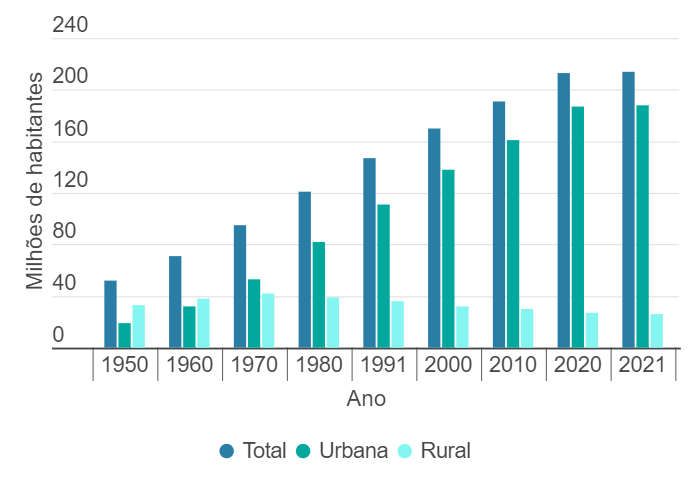
\includegraphics[width=4.25000in,height=2.92013in]{./imgSAEB_9_CHUM6/media/image2.png}
\caption{Gráfico, Gráfico de barras Descrição gerada automaticamente}
\end{figure}

\fonte{~IBGE.}

Tendo em vista o gráfico, aponte dois fatores responsáveis pela mudança
da configuração populacional brasileira a partir dos anos de 1970.

\reduline{A partir dos anos de 1970, o Brasil passou a ter maior parte da população
vivendo em ambiente urbano, concluindo o processo do êxodo rural, em razão da industrialização em vigor no país, que aumentava os postos de
trabalho nas cidades e oferecia diferentes condições de vida, além da
mecanização do campo, que reduzia as possibilidades de trabalho no
ambiente rural.}

\num{5} Leia o trecho a seguir.

\begin{quote}
Aqui a população que reside nas cidades passou de 45\% em 1960 para 75\%
em 1990 e mais de 80\% em 2000. Essa transferência intensa para as
cidades foi fruto de uma política desenvolvimentista implementada a
partir da década 50. A entrada de tecnologia e capital financeiro
imprimiu um novo ritmo à economia brasileira, e progressivamente a
população foi se transferindo para as cidades. O setor agrário da
economia, sobretudo a partir da década de 70, mecanizou-se, liberou mão
de obra e as cidades sofreram um crescimento demográfico repentino.
\end{quote}

\fonte{Jurandyr Ross.~A~sociedade~industrial~e~o~ambiente.
In:~\emph{Geografia~do~Brasil}.~São~Paulo:~EDUSP, 2019.}

Com base no texto, você concorda com a ideia de que o crescimento
demográfico das cidades brasileiras foi acompanhado de amplo
planejamento urbano estatal? Explique seus argumentos com exemplos.

\reduline{Espera-se que o aluno não concorde com a afirmativa, dado que o
crescimento demográfico urbano no Brasil não foi acompanhado com
políticas públicas de ordenamento territorial e de outros tipos.
Como exemplo, tem-se o crescimento numérico e espacial de favelas, mostrando
a insuficiência da política habitacional brasileira, além da
insuficiência dos serviços associados ao saneamento básico --- água
tratada, coleta e tratamento de esgoto, etc.}

\num{6} Analise a imagem a seguir.

%Inserir imagem mostrando a linha cronológica do agronegócio brasileiro.
\fonte{https://www.embrapa.br/visao-de-futuro/trajetoria-do-agro}

\begin{figure}
\centering
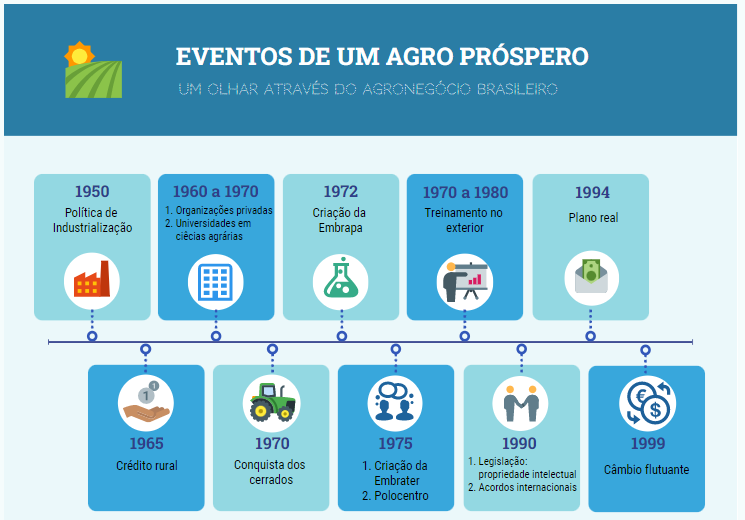
\includegraphics[width=5.04002in,height=3.51806in]{./imgSAEB_9_CHUM6/media/image3.png}
\caption{Linha do tempo Descrição gerada automaticamente}
\end{figure}

A partir da cronologia explicitada na imagem, cite e explique uma
mudança relacionada à produção agrícola brasileira.

\textbackslash{}reduline\{O processo de mecanização e internacionalização
da produção agrícola nacional orientou os cultivos à produção de
\emph{commodities} agrícolas, em detrimento de culturas agrícolas
consumidas no mercado interno. É importante ressaltar que a produção de
\emph{commodities} visava ao direcionamento ao mercado externo.

\num{7} Leia o trecho a seguir.

\begin{quote}
As atividades agrícolas chamadas modernas são cada vez mais avançadas
tecnologicamente, empregando baixa quantidade de mão de obra e
utilizando maquinarias, adubos químicos, inseticidas e herbicidas. Esse
modelo de produção agrícola intensificou-se principalmente nas décadas
que sucederam à Segunda Guerra Mundial. É um modelo de países
industrializados, como Estados Unidos, Inglaterra, França, Alemanha,
Rússia e Ucrânia.
\end{quote}

\fonte{Jurandyr Ross.~A~sociedade~industrial~e~o~ambiente.
In:~\emph{Geografia~do~Brasil}.~São~Paulo:~EDUSP, 2019.}

Você concorda com a ideia de que a modernização agrícola tem favorecido
a concentração fundiária e o processo de saída populacional do campo?
Explique.

\reduline{Espera-se que o aluno concorde com a afirmativa, uma vez que a
modernização agrícola favorece a perda de postos de trabalho, o que
diminui as possibilidades dos trabalhadores rurais, sendo uma
alternativa a saída do campo. Além disso, a modernização também tem
favorecido a concentração fundiária, dada a orientação da produção ao
mercado externo, além da melhor implementação dos insumos agrícolas citados em grandes extensões de terras.}

\num{8} Massimo Montanari e Jean Louis Fladrin, no livro \emph{A
história da alimentação}, consideram que a Revolução Industrial atingiu
a história da gastronomia em vários aspectos, mas antes de tudo pelo
desenvolvimento promovido no setor. A partir dessa ideia, cite duas
mudanças nos hábitos alimentares tendo em vista a industrialização da
gastronomia.

\reduline{Os alunos podem citar o aumento do consumo de alimentos à base de óleo, farinha e açúcar, que tiveram ampla produção com a industrialização. Além disso, houve a redução do consumo de produtos \textit{in natura}, como vegetais e legumes.}

\num{9} Leia o texto.

\begin{quote}
Durante o período de 1960 a 2017, observou-se um aumento significativo
no número de tratores por mil hectares, passando de 0,06 para 17,1
tratores por hectare. Além disso, a potência média por hectare aumentou
de 0,38 para 1,71 cavalo por hectare. De acordo com os autores, houve um
crescimento acentuado no número de tratores (50\%) entre os censos de
2006 e 2017, o que sugere uma forte modernização no setor agropecuário
nesse período.
\end{quote}

\fonte{de pesquisa: Embrapa. Trajetória do Agro.
Disponível em:
https://www.embrapa.br/visao-de-futuro/trajetoria-do-agro. Acesso em: 12
mar. 2023}

A partir do texto, aponte e explique duas consequências do avanço da
modernização do campo.

\reduline{As consequências compreendem a perda de postos de trabalho, dada a
utilização de maquinário, e, consequentemente, a menor utilização de
mão de obra humana, além do aumento da produtividade agrícola.}

\num{10} Leia o trecho a seguir.

\begin{quote}
O processo de industrialização da agricultura tem eliminado
gradativamente a separação entre a cidade e o campo, entre o rural e o
urbano, unificando-os dialeticamente. Isso quer dizer que campo e
cidade, cidade e campo formam uma unidade contraditória.
\end{quote}

\fonte{Ariovaldo~Umbelino
Oliveira.~Agricultura~brasileira:~transformações~recentes.~In:~\emph{Geografia~do~Brasil}.~São~Paulo:~EDUSP,
2019.}

Com base no texto, a partir de seu conhecimento sobre o assunto, aponte
duas situações que ilustram a eliminação gradativa da separação entre
campo e cidade.

\reduline{Duas situações que podem ser expostas compreendem a própria
industrialização da agricultura, que, historicamente, foi tida como uma
atividade urbana e que agora tem sido um motivador do crescimento
urbano no espaço rural, e as mobilizações feitas pelos trabalhadores rurais no espaço urbano.}

\section{Treino}

\num{1} Leia o texto.

\begin{quote}
\textbf{O impacto do ChatGPT e a visão otimista dos especialistas sobre
empregos}
\end{quote}

\begin{quote}
A habilidade avançada do ChatGPT em gerar texto é frequentemente
comparada a um superpoder, gerando preocupações de que possa tornar
muitas profissões obsoletas. No entanto, especialistas entrevistados
pela CNN Portugal acreditam que essa tecnologia pode ser uma
oportunidade para que os trabalhadores desenvolvam novas habilidades e
competências, embora não descartem a possibilidade de algumas profissões
serem afetadas.

Devido à sua capacidade de gerar e analisar texto, o ChatGPT pode ter
impacto em diversas profissões. Por outro lado, ele pode também permitir
que os trabalhadores realizem tarefas rotineiras com mais eficiência e
se concentrem em outras partes mais criativas e complexas de seus
trabalhos.

Os especialistas têm uma visão mais otimista sobre o impacto da
tecnologia nos empregos. Pedro Amorim, Diretor Executivo da Experis,
refere-se ao ChatGPT como ``inteligência assistida'' em vez de
``inteligência artificial'', afirmando que a tecnologia pode fornecer
condições para que os seres humanos desenvolvam novas habilidades e se
concentrem na qualidade, em vez de quantidade.
\end{quote}

\fonte{de pesquisa: João Guerreiro Rodrigues. CNN
Portugal. Inteligência artificial. O ChatGPT põe em perigo a minha
profissão? ``Vão surgir novas funções''. Disponível em:
https://cnnportugal.iol.pt/inteligencia-artificial/emprego/inteligencia-artificial-o-chatgpt-poe-em-perigo-a-minha-profissao-vao-surgir-novas-funcoes/20230121/63cb04ff0cf2c84d7fc429dd.
Acesso em: 11 mar. 2023.}

De acordo com o texto, a inteligência artificial tem o potencial de

\begin{enumerate}
\def\labelenumi{\alph{enumi})}
\tightlist
\item
  renovar a mão de obra.
\item
  reduzir o desemprego estrutural.
\item
  reforçar potencialidades humanas.
\item
  retomar postos de trabalho manual.
\end{enumerate}

BNCC: EF09GE11 -- Relacionar as mudanças técnicas e científicas
decorrentes do processo de industrialização com as transformações no
trabalho em diferentes regiões do mundo e suas consequências no Brasil.

a) Incorreta. No texto, não se destaca a possibilidade de renovação da
mão de obra por conta da introdução de tecnologias no ambiente de
trabalho.

b) Incorreta. No texto, não se fala de desemprego estrutural.

c) Correta. Os especialistas mencionados no texto acreditam no potencial
que a inteligência artificial tem de reduzir a sobrecarga humana com
ações rotineiras, o que abriria espaço para que o ser humano desenvolva
outras potencialidades.

d) Incorreta. Pelo contrário, a introdução de tecnologias no ambiente de
trabalho tende a reduzir postos de trabalho tidos como manuais.

\num{2} Leia o texto.

\begin{quote}
\textbf{Tecnologia aumenta produtividade agropecuária e diminui mão de
obra}
\end{quote}

\begin{quote}
A produção das atividades agropecuárias atingiu R\$ 465,5 bilhões em
2017, sendo 66,2\% (R\$ 308 bilhões) relativos à produção vegetal e
33,8\% (R\$ 157,4 bilhões) da produção animal. Da produção vegetal, 77\%
vêm das lavouras temporárias, 13\% das lavouras permanentes, 5,7\% da
silvicultura, 2,8\% da horticultura, 0,7\% da extração vegetal e 0,6\%
da floricultura. A produção animal se divide em 70,5\% de grande porte,
19\% de aves, 8\% de animais de médio porte e 2,5\% para os de pequeno
porte.
\end{quote}

\begin{quote}
Os dados estão no Censo Agropecuário 2017, divulgado {[}\ldots{}{]} pelo
Instituto Brasileiro de Geografia e Estatística (IBGE). A pesquisa fez
uma fotografia do campo brasileiro no dia 30 de setembro de 2017, com
dados relativos ao período entre 1º de outubro de 2016 e a data base.
\end{quote}

\begin{quote}
O levantamento mostra que a área plantada não aumentou
significativamente, porém a produção foi muito maior. Por exemplo, o
rendimento em quilos por hectare plantado em algodão herbáceo passou de
2,9 mil em 2006 para 4,1 mil em 2017, a soja subiu de 2,5 mil para 3,3
mil, o milho passou de uma produtividade de 3,5 mil quilos por hectare
para 5,5 mil, o arroz foi de 4 mil para 6,4 mil e o feijão subiu de 734
para mil quilos por hectare plantado.
\end{quote}

\begin{quote}
{[}\ldots{}{]}
\end{quote}

\fonte{Akemi Nitahara. Agência Brasil. Tecnologia aumenta
produtividade agropecuária e diminui mão de obra. Disponível em:
https://agenciabrasil.ebc.com.br/geral/noticia/2019-10/tecnologia-aumenta-produtividade-agropecuaria-e-diminui-mao-de-obra.
Acesso em: 10 mar. 2023.}

A partir da leitura do texto, apreende-se que a mecanização das
atividades agrícolas tem

\begin{enumerate}
\def\labelenumi{\alph{enumi})}
\item
  retirado postos de trabalho no campo.
\item
  aumentado a produtividade dos trabalhadores.
\item
  ampliado as possibilidades laborais de atuação no campo.
\item
  reforçado a permanência dos trabalhadores do campo no meio rural.
\end{enumerate}

BNCC: EF09GE11 -- Relacionar as mudanças técnicas e científicas
decorrentes do processo de industrialização com as transformações no
trabalho em diferentes regiões do mundo e suas consequências no Brasil.

a) Correta. Concomitantemente à ampliação da mecanização do campo,
percebe-se que ocorre a redução dos postos de trabalho, ou seja, as
máquinas têm reduzido a necessidade da mão de obra no campo.

b) Incorreta: No texto, ressalta-se o aumento da produtividade, mas isso
não está associado aos trabalhadores em si.

c) Incorreta. Pelo contrário, percebe-se que a mecanização tem sido um
dos motivos da diminuição dos postos de trabalho no campo.

d) Incorreta. Pelo contrário, a perda de postos de trabalho tem sido um
dos fatores de expulsão da população do meio rural brasileiro.

\num{3} Leia o texto

\begin{quote}
A urbanização do Brasil foi impulsionada pelo êxodo rural no passado.
Durante o período de 1950 a 1960, ele contribuiu com 17,4\% do
crescimento populacional das cidades, e continuou sendo um fator
significativo nas duas décadas seguintes.
\end{quote}

\fonte{Texto escrito para este material.}

Entre os fatores que reforçaram esse tipo de migração no país, estão

\begin{enumerate}
\def\labelenumi{\alph{enumi})}
\item
  a mecanização do campo e a concentração fundiária.
\item
  a redução das áreas urbanas e a política de cercamento agrário.
\item
  o estímulo à produção de \emph{commodities} agrícolas e a luta pela
  reforma agrária.
\item
  a internacionalização da produção do campo e o desincentivo à
  industrialização nacional.
\end{enumerate}

BNCC: EF09GE12 -- Relacionar o processo de urbanização às transformações
da produção agropecuária, à expansão do desemprego estrutural e ao papel
crescente do capital financeiro em diferentes países, com destaque para
o Brasil.

a) Correta. O êxodo rural brasileiro foi impulsionado pela mecanização
do campo, que foi retirando postos de trabalho no meio rural, e pela
histórica concentração das terras, que limita as possibilidades de
permanência no campo.

b) Incorreta. No período, não houve redução da área urbana no país, além
de não ter havido uma política de cercamento agrário.

c) Incorreta. Embora tenha havido o estímulo da produção de
\emph{commodities} agrícolas no período, especialmente nos anos 1980, a
luta pela reforma agrária compreende uma forma de permanência no espaço
rural, e não de saída.

d) Incorreta. Embora tenha havido a internacionalização da produção do
campo, não houve o desincentivo à industrialização nacional.



\chapter{SIMULADO 1}

\num{1} Leia o texto.

\begin{quote}
Carvão é o nome dado a diversas rochas sedimentares passíveis
de uso como combustível, constituídas de um material heterogêneo
originado de restos vegetais depositados em águas rasas, protegidos da
ação do oxigênio do ar. {[}...{]}

A extração do carvão pode ser em minas a céu aberto ou
subterrâneas, dependendo da profundidade em que se encontra a camada. As
minas a céu aberto exercem significativo impacto ambiental em razão dos
elementos químicos contidos no carvão, como o enxofre.

Numerosas áreas de mineração antigas no sul do Brasil, trabalhadas
em uma época em que a preocupação com o ambiente natural era muito menor
que atualmente, foram muito degradadas e precisaram ser recuperadas,
trabalho que vem sendo feito nas últimas décadas.

{[}...{]}

\fonte{Serviço Geológico do Brasil. Carvão mineral. Disponível em:
\emph{http://www.cprm.gov.br/publique/SGB-Divulga/Canal-Escola/Carvao-Mineral-2558.html}.
Acesso em: 28 fev. 2023.}
\end{quote}

É possível identificar que o principal impacto da extração de carvão se dá pela

\begin{escolha}
\item
  emissão local de fumaça.
\item
  geração de ilhas de calor.
\item
  exaustão do lençol freático.
\item
  remoção da estrutura superficial do solo.
\end{escolha}

\reduline{BNCC: EF09GE18 -- Identificar e analisar as cadeias industriais e de
inovação e as consequências dos usos de recursos naturais e das diferentes fontes de energia (tais como termoelétrica, hidrelétrica, eólica e nuclear) em diferentes países.

a) Incorreta. A extração do carvão não produz massiva emissão de fumaça.
b) Incorreta. As ilhas de calor são fenômenos associados a grandes
  cidades.
c) Incorreta. Ao contrário da mineração de metais, não se utiliza água
  para a extração de carvão mineral.
d) Correta. Para extrair o carvão, toda a superfície acima da mina precisa
  ser removida.}

\num{2} Analise o esquema.

%\begin{figure}[htpb!]
%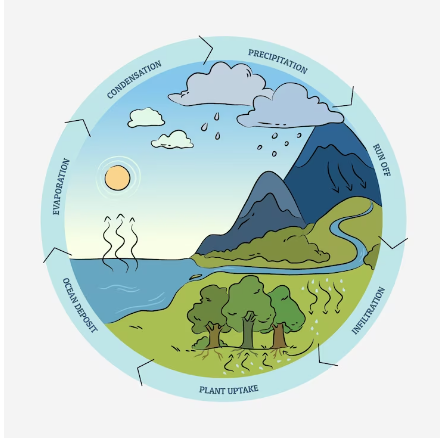
\includegraphics[width=4.58333in,height=4.56250in]{./imgs/img9.png}
%\caption{Fonte:
%https://br.freepik.com/vetores-gratis/informacoes-desenhadas-a-mao-sobre-o-ciclo-da-agua\_18980469.htm\#query=ciclo\%20da\%20agua\&position=1\&from\_view=keyword\&track=ais.}
%\end{figure}
%Paulo, trocar foto: https://br.freepik.com/vetores-gratis/desenho-a-mao-de-um-ciclo-de-agua-de-design-plano_18773933.htm#query=informacoes%20desenhadas%20a%20mao%20sobre%20o%20ciclo%20da%20agua&position=2&from_view=search&track=ais

No ciclo da água, a absorção de energia ocorre

\begin{escolha}
\item
  no escoamento.
\item
  na precipitação.
\item
  na condensação.
\item
  na evaporação.
\end{escolha}

\reduline{BNCC: EF09GE18 -- Identificar e analisar as cadeias industriais e de
inovação e as consequências dos usos de recursos naturais e das diferentes fontes de energia (tais como termoelétrica, hidrelétrica, eólica e nuclear) em diferentes países.

a) Incorreta. O escoamento é orientado pela força da gravidade, e não pela
  energia solar.
b) Incorreta. A precipitação é o efeito da perda de calor por parte das
  nuvens, pois, ao perder calor, o vapor de água condensa-se em pequenas
  gotículas formando nuvens e posteriormente chuva.
c) Incorreta. Ao perder calor, o vapor de água condensa-se em pequenas
  gotículas formando nuvens e posteriormente chuva;
d) Correta. A evaporação é o efeito do ganho de calor (por meio da absorção da energia solar) por parte da água
  líquida, o que gera sua evaporação..}

\num{3} Leia o texto.

\begin{quote}
\textbf{Capacidade de geração de energia eólica deve bater recorde neste ano}

O Brasil registra, até fevereiro [de 2023], 890 parques eólicos instalados em 12 estados brasileiros. Eles somam 25,04 gigawatts (GW) de capacidade instalada em operação comercial, que beneficiam 108,7 milhões de habitantes.

Desse total, 85\% estão na Região Nordeste. De acordo com a Associação Brasileira de Energia Eólica (Abeeólica), até 2028 o Brasil terá 44,78 GW de capacidade instalada desse tipo de energia, cuja participação na matriz nacional atinge, atualmente, 13,2\%. A eólica já responde hoje por 20\% da geração de energia [de] que o país precisa.

No ano passado, o setor bateu recorde de 4 GW instalados e, para este ano, a presidente executiva da Abeeólica, Elbia Gannoum, espera atingir novo recorde, superando esse número. “Encerrando 2023, estaremos com 29 GW de capacidade instalada. Essa é a nossa previsão em termos de potência, e isso é superior a R\$ 28 bilhões, porque cada gigawatt de eólica instalada é da ordem de R\$ 7 bilhões”, disse Elbia {[}...{]}.

\fonte{Alana Gandra. Agência Brasil. Capacidade de geração de energia eólica deve bater recorde neste ano. Disponível em:
\emph{https://agenciabrasil.ebc.com.br/economia/noticia/2023-04/capacidade-de-geracao-de-energia-eolica-deve-bater-recorde-neste-ano}.
Acesso em: 05 abr. 2023.}
\end{quote}

O texto demonstra que o Brasil

\begin{escolha}
\item
  está avançando na produção de energia de uma fonte renovável.
\item
  é dependente de um tipo de energia que não tem muito potencial no país.
\item
  produz mais energia eólica do que a de qualquer outro tipo.
\item
  tem aumentado a produção de energia de fonte não renovável.
\end{escolha}

\reduline{BNCC: EF09GE18 -- Identificar e analisar as cadeias industriais e de
inovação e as consequências dos usos de recursos naturais e das
diferentes fontes de energia (tais como termoelétrica, hidrelétrica,
eólica e nuclear) em diferentes países.

a) Correta. O texto demonstra o aumento da produção de energia eólica, que é de uma fonte renovável.
b) Incorreta. O texto demonstra que o Brasil tem muito potencial para energia eólica.
c) Incorreta. O texto demonstra que a energia eólica ainda corresponde a uma parcela pequena da matriz energética brasileira.
d) Incorreta. O texto demonstra o aumento de produção de energia de uma fonte renovável.}

\num{4} Leia o texto.

\begin{quote}
\textbf{Cota racial}

Em vigor desde 10 de junho de 2014, a Lei 12.990 prevê uma cota de vagas para negros e pardos em concursos públicos, com o objetivo de reduzir as desigualdades sociais, econômicas e educacionais entre as raças e promover uma maior inclusão e diversidade nos cargos públicos.

\fonte{Jusbrasil. Entenda como funciona a "cota racial" para concursos públicos no Brasil. Disponível em: \emph{https://www.jusbrasil.com.br/artigos/entenda-como-funciona-a-cota-racial-para-concursos-publicos-no-brasil/243608268}. Acesso em: 04 maio 2023.}
\end{quote}

Tal como em vestibulares, as cotas nos concursos públicos buscam

a)  discriminar racialmente a população branca.

b)  conferir privilégios para minorias demográficas.

c)  compor uma política ampla de reparação histórica.

d)  estabelecer mecanismos de compensação para incapazes.

\reduline{BNCC: EF09HI03 -- Identificar os mecanismos de inserção dos
negros na sociedade brasileira pós-abolição e avaliar os seus
resultados.

a)  Incorreta. As políticas de cotas não versam sobre a população
    branca; apenas beneficiam a população negra e mais pobre.
b)  Incorreta. Ainda que fosse uma política de privilégios, a população
    foco não é minoritária, pois os negros compõem maioria demográfica.
c)  Correta. As leis de cotas buscam reparar injustiças históricas
    cometidas contra a população negra, que, por exemplo, sequer teve
    direito a trabalho livre após o fim da escravidão, o que causou
    inúmeras consequências relacionadas à exclusão econômica dessa
    população. 
d)  Incorreta. Essa alternativa possui uma abordagem racista ao afirmar
    que a população negra é menos capaz que a população branca.}


\num{5} Leia o texto.

\begin{quote}
\textbf{ONGs apontam racismo em falta de políticas públicas em áreas de risco}

A falta de políticas públicas voltadas a atender à demanda da população negra e periférica que vive em áreas de risco ambiental –-- como nos locais atingidos por deslizamentos de terra no litoral Norte de São Paulo --- é uma opção das administrações públicas e demonstra racismo ambiental. A avaliação é de especialistas de duas organizações da sociedade civil, o Greenpeace e o Instituto Polis.

``[O racismo ambiental] está muito ligado à segregação e [à] exclusão em relação ao direito de ter o meio ambiente de determinada região equilibrado. A gente observa a escolha política, o critério para definir locais que vão ter políticas públicas. E elas não conseguem chegar sempre à população dos morros, negra e periférica'', afirma Rodrigo Jesus, da Campanha Clima e Justiça, do Greenpeace.

De acordo com ele, a falta de prioridade das populações negra e periférica demonstra ainda negligência. {[}...{]}

\fonte{Bruno Bocchini. Agência Brasil. ONGs apontam racismo em falta de políticas públicas em áreas de risco. Disponível em: \emph{https://agenciabrasil.ebc.com.br/geral/noticia/2023-02/ongs-apontam-racismo-em-falta-de-politicas-publicas-em-areas-de-risco}. Acesso em: 04 maio 2023.}
\end{quote}

A criação de canais de representação e participação popular da população
negra contribuiria para a diminuição de desastres ambientais de maneira
geral ao

a)  organizar os governos locais.
b)  valorizar pautas esquecidas no debate público.
c)  explicar os mecanismos dos desastres ambientais.
d)  adequar o orçamento dirigido a obras públicas pontuais.

\reduline{BNCC: EF09HI04 -- Discutir a importância da participação da
população negra na formação econômica, política e social do Brasil.

a) Incorreta. Atualmente existe extensa estrutura jurídica que embasa
a organização dos governos, não sendo este o fator causador da baixa
expressão política da população periférica.
b) Correta. Por serem as mais afetadas e, ao mesmo tempo, as menos
representadas, as pautas da população negra são pouco discutidas no
debate público; assim, a criação de canais de expressão e participação
popular daria mais evidência às pautas que afetam a população negra e
periférica.
c) Incorreta. Os mecanismos de desastres ambientais já são bem conhecidos,
e o problema repousa nas atitudes que deveriam ser, mas não são tomadas para
evitá-los, o que se explica em parte por racismo institucional.
d) Incorreta. A questão pede uma contribuição para a solução do conjunto
dos problemas ambientais que afetam a população negra, e não intervenções
pontuais.}


\chapter{SIMULADO 2}

\num{1} Leia o texto.

\begin{quote}
\textbf{O arado}

Por volta do ano 5000 a.C., o ser humano
teria deixado de vagar atrás de terras
para cultivo e já começava a domesticar
animais. Foi nesse contexto que surgiu um
instrumento feito com galhos bifurcados e
uma pedra afiada na ponta, que servia
para arar a terra. Segundo especialistas,
a invenção do arado é um marco da Revolução Agrícola, que permitiu o ser humano fixar-se em aldeias, aumentar sua produtividade e dar início a atividades comerciais.

\fonte{Fonte de pesquisa: Superinteressante. Arado. Disponível em: \emph{https://super.abril.com.br/comportamento/arado/}. Acesso em: 04 abr. 2023.}
\end{quote}

No contexto apresentado, o arado cumpria a função de

\begin{escolha}
\item
  otimizar o trabalho humano.
\item
  domesticar os animais.
\item
  criar redes de água.
\item
  limpar terrenos.
\end{escolha}

\reduline{BNCC: EF09GE05 -- Analisar fatos e situações para compreender a
integração mundial (econômica, política e cultural), comparando as
diferentes interpretações: globalização e mundialização.

a) Correta. O arado começou a ser utilizado para diminuir o tempo gasto com o preparo e a semeadura do solo; assim  constitui um instrumento que
otimiza o trabalho humano, isto é, a transformação de recursos naturais
em produtos com valor de uso. b) Incorreta. O arado não foi usado para domestificar animais, mas começou a ser empregado com o auxílio de animais domesticados.
c) Incorreta. O arado é um instrumento de preparação do solo para plantio.
d) Incorreta. O arado é empregado em terrenos já disponibilizados ao
plantio.}

\num{2} Leia os textos.

\textbf{TEXTO 1}
\begin{quote}
\textbf{Processo de desindustrialização no Brasil se acentua}

A indústria brasileira dá sinais de que algo de errado acontece no
setor. Do início do ano [de 2021] até agora [ou seja, março de 2021], três gigantes multinacionais
anunciaram que vão abandonar o Brasil. A norte-americana Ford deixa o
mercado de fabricação de veículos nacional depois de mais de 100 anos. A
alemã Mercedes-Benz fecha a única fábrica no Brasil de carros de luxo. A
japonesa Sony fecha a fábrica em Manaus (AM) e abandona o mercado de
televisores, câmeras e aparelhos de áudio. Esse movimento mostra que o
País passa por um processo de desindustrialização, e não é de hoje, como
sugerem alguns números e apontam especialistas.

{[}...{]}

\fonte{Ferraz Jr. Jornal da USP. Processo de desindustrialização no Brasil se
acentua. Disponível em:
\emph{https://jornal.usp.br/atualidades/processo-de-desindustrializacao-no-brasil-se-acentua/}.
Acesso em: 22 fev. 2023.}
\end{quote}

\textbf{TEXTO 2}
\begin{quote}
\textbf{Exportações do agronegócio batem recorde em dezembro e no ano de 2021}

As exportações do agronegócio alcançaram valores recordes para o
mês de dezembro passado e também para o ano de 2021. Foram US\$ 9,88
bilhões, valor recorde para os meses de dezembro: 36,5\% superior aos
US\$ 7,24 bilhões de 2020. Em 2021, o total exportado com o agronegócio
resultou em US\$ 120,59 bilhões, alta de 19,7\%, em relação ao ano
anterior, conforme dados divulgados nesta quinta-feira [13/01/2022] pela
Secretaria de Comércio e Relações Internacionais (SCRI) do Ministério da
Agricultura, Pecuária e Abastecimento (Mapa).

{[}...{]}

\fonte{Ministério da Agricultura e Pecuária. Exportações do agronegócio batem recorde em dezembro e no ano de 2021. Disponível em: \emph{www.gov.br/agricultura/pt-br/assuntos/noticias/exportacoes-do-agronegocio-batem-recorde-em-dezembro-e-no-ano-de-2021}. Acesso em: 22 fev. 2023.}
\end{quote}

Associando-se os textos, é possível diagnosticar que, no contexto
globalizado atual, o Brasil tem se constituído como

\begin{escolha}
\item
  exportador de serviços e consumidor de \textit{commodities}.
\item
  investidor tecnológico e consumidor de industrializados.
\item
  exportador de produtos básicos e consumidor de tecnologia.
\item
  centralizador da indústria global e exportador de produtos básicos.
\end{escolha}

\reduline{BNCC: EF09GE05 -- Analisar fatos e situações para compreender a
integração mundial (econômica, política e cultural), comparando as
diferentes interpretações: globalização e mundialização.

a) Incorreta. O setor de serviços constitui destaque interno no Brasil.
b) Incorreta. A desindustrialização demonstra que o Brasil passa por um
  processo de perda de tecnologia, seja por perder empresas detentoras
  de tecnologias, seja por não investir na tecnologia, setor que anda
  lado a lado com o desenvolvimento industrial.
c) Correta. O recorde de exportações agrícolas revela o pleno
  desenvolvimento do setor no país, o que mostrar que o Brasil tem se
  especializado na produção de itens básicos classificados como
  matéria-prima (\textit{commodities}), e essa configuração econômica
  contribui para o país ficar dependente de tecnologia externa, já que o
  desenvolvimento tecnológico, mesmo para máquinas agrícolas, parte do
  setor industrial.
d) Incorreta. Em um dos textos, menciona-se a perda crônica de empresas
  industriais.}

\num{3} 

\begin{quote}
\textbf{Sem fé, lei ou rei}
No século XVI, Pero de Magalhães (um cronista português) acreditava ter encontrado a chamada \textit{mácula original do silvícola brasileiro}. O cronista escreveu que os indígenas estavam fadados a não se destacar, o que se devia ao fato de que, na língua deles, não havia F, L ou R, de modo que não tinham nem fé, nem lei, nem rei.

\fonte{Terras indígenas no Brasil. Sem fé, lei ou rei. Disponível em:
\emph{https://terrasindigenas.org.br/noticia/30695}. Acesso em: 22 fev. 2023.}
\end{quote}

A fala de Pero Magalhães é um demonstrativo de que a sociedade tida como
correta, em sua visão, teria como base

\begin{escolha}
\item
  a ausência da figura do rei.
\item
  a adoção da língua portuguesa.
\item
  a ideia de proteção ambiental dos indígenas.
\item
  as características políticas e sociais da Europa.
\end{escolha}

\reduline{BNCC: EF09GE06 -- Associar o critério de divisão do mundo em Ocidente e
Oriente com o Sistema Colonial implantado pelas potências europeias.

a) Incorreta. Não apenas a ausência da figura do monarca é criticada, mas
também a ausência da fé cristã e da lei europeia.
b) Incorreta. O centro da visão colonialista não estava na língua falada,
mas nas características culturais diferenciadas dos povos indígenas.
c) Incorreta. A fala do cronista do português não se caracteriza por um tom de cuidado com os indígenas.
d) Correta. A monarquia, a fé cristã como instituição de estado e
a legislação portuguesa são encaradas como base de uma civilização
correta na fala de Pero Magalhães, motivo pelo qual ele critica a ausência
desses elementos entre os indígenas.}

\num{4} Analise o mapa.

\begin{quote}
\textbf{Ilú Obá De Min}

A associação Ilú Obá De Min é uma entidade sem fins lucrativos de São Paulo que tem como foco o trabalho com culturas de matriz africana, afro-brasileira e a valorização da mulher. Fundada em 2004 pelas percussionistas Beth Beli, Adriana Aragão e Girlei Miranda, a associação se tornou uma pessoa jurídica em 2006. Seu principal objetivo é preservar e divulgar a cultura negra no Brasil e fortalecer a participação e representatividade das mulheres negras. O projeto mais reconhecido da entidade é o Bloco Afro Ilú Oba De Min, cuja bateria é formada exclusivamente por mulheres. Desde 2005, o bloco realiza cortejos pelas ruas de São Paulo, honrando e celebrando a cultura afro-brasileira, além de destacar a participação e protagonismo feminino. Os cortejos do Bloco são uma grande intervenção cultural que promove a cultura negra, a cultura popular e a participação ativa das mulheres na sociedade por meio da arte. A iniciativa também traz para as áreas urbanas diversas manifestações da cultura negra, como o maracatu, batuque, coco, jongo, entre outras.

\fonte{Fonte de pesquisa: Ilú Obá De Min. Quem somos. Disponível em: \emph{https://iluobademin.com.br/institucional/quem-somos/}. Acesso em: 06 mar. 2023.}
\end{quote}

As ações executadas pela associação Ilú Obá De Min objetivam

a)  naturalizar as expressões culturais negras como identidade
    sociocultural.
b)  dramatizar as expressões culturais negras como meras atitudes
    lúdicas.
c)  diferenciar as expressões culturais negras como práticas
    estrangeiras.
d)  promover atos de protesto pontuais contra o racismo persistente.

\reduline{BNCC: EF09GE03 -- Identificar diferentes manifestações
culturais de minorias étnicas como forma de compreender a multiplicidade
cultural na escala mundial, defendendo o princípio do respeito às
diferenças.

a)  Correta. A construção de projetos culturais de matrizes
    afro-brasileiras demonstra que as manifestações culturais promovidas
    pela associação têm como objetivo resgatar e consolidar uma
    identidade cultural própria da população negra.
b)  Incorreta. Os projetos desenvolvidos não têm como foco o
    divertimento, e sim a construção de práticas que representam a
    socialização da população negra em uma matriz cultural de origem
    africana.
c)  Incorreta. A associação busca a naturalização e a cotidianização das
    expressões culturais negras, o que promoveria maior integração
    dessas práticas com a cultura nacional.
d)  Incorreta. O objetivo da associação é a valorização das expressões
    culturais negras, que não são utilizadas como uma forma de
    contestação da ordem, mas como instrumento de consolidação de
    práticas socioculturais de origem africana}

\num{5}

\begin{quote}
\textbf{Brasil é líder em mortes de ambientalistas na última década}

Nos últimos 10 anos, o Brasil liderou o ranking mundial de assassinatos de defensores e defensoras do meio ambiente. De acordo com registros globais de 2012 a 2021, das 1.733 mortes, 342 ocorreram no país, representando quase 20\% do total. Entre as vítimas estão Maria José Rodrigues, de 78 anos, e seu filho José do Carmo Correa Junior, que foram esmagados por uma palmeira derrubada por um trator enquanto coletavam coco de babaçu em Penalva, Maranhão, em novembro de 2021. O tratorista estava desmatando uma área que já havia sido assegurada para uma comunidade tradicional, mas que estava sendo invadida a mando de um fazendeiro que, segundo denúncias dos moradores, pretendia plantar capim no terreno.

\fonte{Fonte de pesquisa: Nádia Pontes. G1. Brasil é líder em mortes de ambientalistas na última década. Disponível em: \emph{https://g1.globo.com/meio-ambiente/noticia/2022/09/29/brasil-e-lider-em-mortes-de-ambientalistas-na-ultima-decada.ghtml}. Acesso em: 04 maio 2023.}
\end{quote}

Qual das alternativas sintetiza as causas de violência contra
ambientalistas como as relatadas?

a)  Invasão de terras públicas.

b)  Disputa por recursos naturais.

c)  Roubo de produção agropecuária.

d)  Desregulamentação do extrativismo.

\reduline{BNCC: EF09HI26 -- Discutir e analisar as causas da violência
contra populações marginalizadas (negros, indígenas, mulheres,
homossexuais, camponeses, pobres etc.) com vistas à tomada de
consciência e à construção de uma cultura de paz, empatia e respeito às
pessoas.

a)  Incorreta. Não há menção no texto à invasão de terras públicas como
    causa de violência.
b)  Correta. As mortes ocorridas em área previamente destinada ao
    extrativismo tradicional demonstram que disputas pelos recursos
    naturais são causas evidentes da violência rural.
c)  Incorreta. Não há menção no texto à prática de roubo da produção
    agropecuária como causa de violência.
d)  Incorreta. No texto, fica claro que a área onde ocorreram as mortes
    era destinada ao extrativismo, ou seja, existe regulamentação da
    atividade.}

\chapter{SIMULADO 3}

\num{1} Leia o texto.

\begin{quote}
\textbf{O caso de injustiça envolvendo a modelo Babiy Querino e a falha na identificação por foto}

Em 2017, a vida de Barbara Querino, então com 22 anos, foi drasticamente alterada por um reconhecimento 
fotográfico irregular. A modelo e dançarina, conhecida como Babiy, foi fotografada por policiais militares 
no dia em que seu irmão e primo foram presos, apesar de não ter qualquer envolvimento com o crime. A foto 
circulou em grupos de WhatsApp e páginas do Facebook, que a apresentaram falsamente como membro de uma 
quadrilha de assaltantes de carros atuando na zona sul de São Paulo. Em janeiro de 2018, Babiy foi presa 
sob acusação de ter participado de dois roubos em setembro de 2017, e permaneceu na prisão por 1 ano e 8 
meses, apesar de apresentar provas da sua inocência. Em 2020, a dançarina finalmente foi absolvida de todas 
as acusações.

\fonte{Caê Vasconcelos. Ponte. Por que tantos negros são alvo de prisão injusta com base em reconhecimentos. Disponível em: \emph{https://ponte.org/por-que-tantos-negros-sao-alvo-de-prisao-injusta-com-base-em-reconhecimentos/}. Acesso em: 10 mar. 2023.}
\end{quote}

Acontecimentos como o relatado são um claro desrespeito à "Declaração
universal dos direitos humanos" porque contrariam o princípio de que ninguém será

a)  mantido em escravidão ou servidão.

b)  preso, detido ou exilado arbitrariamente.

c)  submetido à tortura nem a tratamento cruel.

d)  privado de sua nacionalidade arbitrariamente.

BNCC: EF09HI16 -- Relacionar a Carta dos Direitos Humanos ao processo de
afirmação dos direitos fundamentais e de defesa da dignidade humana,
valorizando as instituições voltadas para a defesa desses direitos e
para a identificação dos agentes responsáveis por sua violação.

a) Incorreta. O texto trata de uma prisão injustas, e não de fatos
análogos à escravidão.
b) Correta. A modelo mencionada no texto foi presa, sem ter praticado
nenhum crime, com base em supostas provas forjadas pelas forças policiais, o
que contraria um dos artigos da ``Declaração universal dos direitos
humanos'', de que ninguém será arbitrariamente preso ou detido ou
exilado.
c) Incorreta. Não há menção a tortura no texto.
d) Incorreta. Não se trata de privação da nacionalidade.


\num{2} Leia o texto.

\begin{quote}
\textbf{Sistemas agroflorestais}

Os Sistemas Agroflorestais (SAFs) permitem aos agricultores familiares conciliar a produção de alimentos com a gestão das riquezas naturais de cada bioma. Na Bahia, {[}...{]} indígenas da etnia Pataxó, do território Barra Velha, município de Porto Seguro, a 629 km de Salvador, receberam do grupo ambiental Natureza Bela apoio para a implantação do corredor ecológico Monte Pascoal-Pau-Brasil, com a recuperação de uma área de mais de 50 hectares de terra, por meio da produção agroecológica de alimentos no Sistema Agroflorestal (SAF). {[}...{]}

\fonte{CONAFER. Agricultores Pataxó aliam produção de alimentos com reflorestamento via SAFs. Disponível em: \emph{https://conafer.org.br/povos-conafer-agricultores-pataxo-aliam-producao-de-alimentos-com-reflorestamento-via-safs/}. Acesso em: 11 mar. 2023.}
\end{quote}

Devido à prática de agricultura ecológica, a população Pataxó necessita,
primordialmente, de

a)  empréstimos bancários.

b)  qualificação na área industrial.

c)  áreas completamente florestadas.

d)  território disponível para plantio.

a) Incorreta. Apesar de empréstimos comporem quase sempre o circuito da
agricultura, a prática agroecológica por si não precisa de empréstimos
para ser efetivada.
b) Incorreta. Como o contexto fala de expansão de cultivos, tal alternativa
não se impõe como uma necessidade.
c) Incorreta. Como se mencionam cultivos, as áreas totalmente florestadas
não seriam úteis.
d) Correta. A população Pataxó precisa de áreas para o plantio, já que,
conforme o texto, estão desenvolvendo cultivos agrícolas.


\num{3} Leia o texto.

\begin{quote}
Nas décadas de 1820 e 1830, o avanço impessoal e poderoso da
máquina e do mercado começou a deixá-los [os trabalhadores pobres] de lado. Na melhor das
hipóteses, este fato fazia com que homens independentes se tornassem
dependentes, e que as pessoas se transformassem em ``mãos''. Na pior das
hipóteses, e a mais frequente, criava multidões de desclassificados,
empobrecidos e famintos tecelões manuais, tecelões mecânicos etc., cuja
miséria gelava o sangue do economista mais insensível.

\fonte{E. Hobsbawm. \textit{A era das revoluções}. São Paulo: Paz e Terra, 2011.}
\end{quote}

De acordo com o texto, o avanço da mecanização industrial na Europa, no
período destacado, foi um responsávelpor

a)  minar as atividades laborais de trabalhadores especializados.

b)  garantir pleno emprego aos trabalhadores urbanos.

c)  incentivar a criatividade no ambiente laboral.

d)  oferecer boas condições de vida.

BNCC: EF09GE10 -- Analisar os impactos do processo de industrialização na
produção e circulação de produtos e culturas na Europa, na Ásia e na
Oceania.

a) Correta. No texto, destaca-se que o avanço da mecanização foi
responsável por destruir a atividade laboral dos trabalhadores
especializados, que detinham o conhecimento da sua produção, como os
tecelões e artesões, uma vez que a indústria potencializou a capacidade
produtiva das mercadorias finais desses trabalhadores.

b) Incorreta. No texto, não se faz menção ao pleno emprego no setor
industrial.

c) Incorreta. Pelo contrário, por se tornarem apenas ``mãos'', os
trabalhadores não tinham mais a possibilidade de criatividade nas
atividades laborais.

d) Incorreta. O texto é enfático ao ressaltar as péssimas condições de
vida de grande parte dos trabalhadores urbanos.

\num{4} Leia o texto.

\begin{quote}
As tensões entre judeus e não judeus atingiram um nível crítico, e em 1948, uma Grã-Bretanha exausta transferiu a questão para as Nações Unidas, que votaram a favor da divisão da região em dois países. Os judeus concordaram, enquanto os árabes manifestaram sua discordância.

\fonte{Texto escrito para este material.}
\end{quote}

A situação apresentada faz referência à disputa

a)  política entre Iraque e Irã.

b)  bélica entre a Síria e o Líbano.

c)  territorial entre Israel e Palestina.

d)  diplomática entre Iêmen e Arábia Saudita.

BNCC: EF09GE08 -- Analisar transformações territoriais, considerando o
movimento de fronteiras, tensões, conflitos e múltiplas regionalidades
na Europa, na Ásia e na Oceania.

a) Incorreta. As relações envolvendo Iraque e Irã não envolvem a
disputa entre judeus e árabes.

b) Incorreta. As relações envolvendo Síria e Líbano não envolvem a
disputa entre judeus e árabes.

c) Correta. Judeus e árabes têm sua disputa mais conhecida envolvendo
a formação do Estado de Israel, judeu, e o impedimento à formação do
Estado da Palestina, árabe. Não bastasse ambos estarem situados no mesmo
território, Israel vem incorporando áreas destinadas aos
palestinos.

d) Incorreta. As relações envolvendo Iêmen e Arábia Saudita não
envolvem a disputa entre judeus e árabes.


\num{5} Leia o texto.

\begin{quote}
\textbf{Os curdos}

Os curdos, descendentes da Pérsia antiga, constituem hoje a maior nação apátrida do mundo, com uma população estimada entre 30 e 40 milhões de pessoas. Sua presença na região montanhosa do Curdistão, que se estende por parte dos territórios de Irã, Iraque, Síria, Armênia e Turquia, remonta a 4.300 a.C. Com cerca de 500 mil quilômetros quadrados, o Curdistão é uma região histórico-cultural habitada pelos curdos. A maior concentração de curdos encontra-se no sudeste turco, com cerca de 20 milhões de pessoas.

\fonte{Fonte de pesquisa: Folha de S.Paulo. Entenda quem são os curdos, povo no centro da disputa entre Turquia e EUA. Disponível em: \emph{https://www1.folha.uol.com.br/mundo/2019/10/entenda-quem-sao-os-curdos-a-maior-nacao-apatrida-do-mundo.shtml}. Acesso em: 05 maio 2023.}
\end{quote}

A característica apátrida do povo curdo denota a ausência de

a)  uma cultura nacional.
b)  um território próprio.
c)  um idioma comum.
d)  um dialeto.

BNCC: EF09GE08 -- Analisar transformações territoriais, considerando o
movimento de fronteiras, tensões, conflitos e múltiplas regionalidades
na Europa, na Ásia e na Oceania.

a)  Incorreta. O termo ``apátrida'' compreende as pessoas que não apresentam uma nacionalidade e não está diretamente relacionado aos aspectos culturais.
b)  Correta. Os curdos são apátridas por não terem o sentimento de pertencimento aos países que habitam, e isso evidencia que os curdos carecem de um território próprio para a formação do seu Estado.
c)  Incorreta. O termo ``apátrida'' compreende as pessoas que não apresentam uma nacionalidade e não está diretamente relacionado aos aspectos linguísticos.
d)  Incorreta. O termo ``apátrida'' compreende as pessoas que não apresentam uma nacionalidade e não está diretamente relacionado aos dialetos locais.


\chapter{SIMULADO 4}

\num{1} Leia o texto.

\begin{quote}
Por volta do século XIX, a Grã-Bretanha havia se tornado o maior produtor mundial de tecidos de algodão, superando a Índia. Isso não ocorreu por acaso, mas sim devido a uma mudança do centro de beneficiamento do algodão da Índia para a Inglaterra. Esse declínio na produção indiana não se deveu à situação política do país, mas sim às conquistas europeias, que trouxeram novas formas de organização do trabalho e tecnologias avançadas.

\fonte{Texto escrito para este material.}
\end{quote}

O texto permite inferir que, em meados do Século XIX, a

a)  Índia manteve o mercado consumidor local dos seus tecidos.

b)  produção inglesa era insuficiente para o mercado consumidor indiano.

c)  produção indiana perdeu em competitividade frente à produção
    inglesa.

d)  Inglaterra não acessou o mercado consumidor de tecidos da região
    do Oceano Índico.

BNCC: EF09GE10 -- Analisar os impactos do processo de industrialização na
produção e circulação de produtos e culturas na Europa, na Ásia e na
Oceania.

a) Incorreta. O texto destaca que o avanço da produção inglesa
``inundou'' o mercado indiano de tecidos.

b) Incorreta. O texto destaca o oposto: a produção inglesa, mais
competitiva, acessou o mercado indiano, minando a produção local de
tecidos.

c) Correta. A ideia de competitividade compreende a
comparação da atividade produtiva de determinado segmento entre dois
locais, considerando-se qual oferece o produto mais barato com menor custo. No caso, a
indústria inglesa era mais competitiva frente à produção de tecidos
indiana, razão pela qual se notou a maior presença dos produtos
industriais.

d) Incorreta. Pelo contrário, o texto destaca a presença de tecidos
ingleses na Índia.


\num{2} Leia o texto.

\begin{quote}
\textbf{Mecanização no campo muda as relações de trabalho}

A introdução de máquinas no campo está transformando as dinâmicas de trabalho no setor agrícola brasileiro. O trabalhador rural que antes era contratado para realizar o plantio e a colheita manual de culturas como cana-de-açúcar, café e algodão, agora está operando máquinas. Consequentemente, o antigo boia-fria migra para setores urbanos, como a construção civil. De acordo com especialistas, o crescimento econômico que acompanha o aumento da produção tem compensado os efeitos da tecnologia no emprego, pois uma única máquina pode substituir mais de 100 trabalhadores.

\fonte{Fonte de pesquisa: Marinella Castro. Estado de Minas. Mecanização no campo muda as relações de trabalho. Disponível em: https://www.em.com.br/app/noticia/economia/2013/01/14/internas\_economia,343131/mecanizacao-no-campo-muda-as-relacoes-de-trabalho.shtml. Acesso em: 05 maio 2023.}
\end{quote}

No caso apontado, a mecanização do campo foi responsável pela

a)  realocação dos trabalhadores.

b)  diminuição dos postos de trabalho.

c)  manutenção de atividades manuais.

d)  flexibilização das atividades laborais.

BNCC: EF09GE12 -- Relacionar o processo de urbanização às transformações
da produção agropecuária, à expansão do desemprego estrutural e ao papel
crescente do capital financeiro em diferentes países, com destaque para
o Brasil.

a) Correta. Os trabalhadores foram realocados para outras
funções, dada a substituição do trabalho manual pelo uso de máquinas.

b) Incorreta. Nesse caso, não houve a perda de postos de trabalho, mas os
trabalhadores apenas foram realocados.

c) Incorreta. Pelo contrário, percebe-se que o trabalho manual foi
substituído pelo uso das máquinas.

d) Incorreta. O texto não destaca algum tipo de flexibilização
laboral.


\num{3} Leia o texto.

\begin{quote}
Em diversas cidades em que a governabilidade é questionável, o Estado frequentemente não é capaz de assegurar a manutenção da lei e da ordem, bem como suprir as necessidades básicas de segurança. Em decorrência disso, diversas alternativas ilegais de sistemas de segurança acabam sendo estabelecidas.

\fonte{Texto escrito para este material.}
\end{quote}

A situação descrita no texto exemplifica

a)  o vácuo de poder deixado pelo Estado.

b)  o gerenciamento popular de demandas comuns.

c)  a concessão de legitimidade ao crime organizado.

d)  a opção deliberada no oferecimento de segurança pública.

BNCC: EF09GE08 -- Analisar transformações territoriais, considerando o movimento de fronteiras,
tensões, conflitos e múltiplas regionalidades na Europa, na Ásia e na Oceania.

a) Correta. A atuação do crime organizado, no caso do oferecimento de
segurança por agentes do crime organizado, dá-se pelo vácuo de poder
deixado pelo Estado e cooptado pelos criminosos. Na ausência de um
agente regulador, os criminosos impõem sua lógica aos habitantes locais,
referendados pelo aparato bélico, que depois utilizam para combater o
próprio Estado e manter o controle territorial.

b) Incorreta. Na situação descrita, não há o envolvimento popular no
controle da segurança oferecida; pelo contrário, a lógica dos criminosos
é imposta, com os populares seguindo suas regras.

c) Incorreta. O crime organizado não tem ações e existência tidas
como legítimas, uma vez que o monopólio da violência pertence somente ao
Estado.

d) Incorreta. Nas áreas de controle do crime organizado, não há uma
opção ou alternativa paralela no oferecimento da segurança.


\num{4} Leia o texto, sobre o Movimento dos Trabalhadores Rurais Sem Terra
(MST).

\begin{quote}
Organizado nacionalmente, ele se constitui no principal
movimento social no campo e busca, através das ocupações de terras,
criar fatos políticos que mobilizem e sensibilizem os governantes para a
necessidade da reforma agrária. Esse movimento utiliza-se também das
caminhadas pelas estradas até as capitais, onde se realizam
manifestações e ocupações de repartições públicas para pressionar os
governos.

\fonte{Ariovaldo Umbelino de Oliveira. Os movimentos sociais no campo e a reforma agrária no Brasil. In: \textit{Geografia do Brasil}. São Paulo: EDUSP, 2019.}
\end{quote}

Depreende-se que a finalidade do movimento social citado compreende a

a)  correção de uma assimetria criada pelo Estado brasileiro ao longo
    do tempo.

b)  promoção de insegurança aos produtores rurais do agronegócio
    nacional.

c)  ampliação das relações entre pequenos e grandes produtores
    agrícolas.

d)  centralização e o direcionamento da produção agrícola nacional.

BNCC: EF09GE08 -- Analisar transformações territoriais, considerando o movimento de fronteiras,
tensões, conflitos e múltiplas regionalidades na Europa, na Ásia e na Oceania.

a) Correta. A reforma agrária no Brasil visa corrigir um aspecto
histórico na estrutura fundiária brasileira, pautada historicamente pelo
latifúndio. Dessa forma, o MST tem como finalidade forçar o Estado
nacional a corrigir uma assimetria fomentada ao longo do tempo.

b) Incorreta. A luta pela reforma agrária no Brasil não visa prejudicar
o agronegócio nacional e, muito menos, promover insegurança
para os produtores.

c) Incorreta. De acordo com o texto, o MST não tem como finalidade
intermediar a relação entre pequenos e grandes produtores agrícolas.

d) Incorreta. De acordo com o texto, o MST não tem como finalidade
centralizar e direcionar a produção agrícola nacional.


\num{5} Leia o texto.

\begin{quote}
\textbf{Ditadura militar contribuiu para genocídio dos povos indígenas}

{[}...{]}

Em depoimento à Comissão Nacional da Verdade, Davi Kopenawa, líder
yanomami, relembrou o descaso do governo durante a realização de grandes
obras. Segundo a liderança, as estradas abriram caminho para os
invasores garimpeiros e fazendeiros.

``Eu não sabia que o governo vinha deixar estrada na terra yanomami. A
autoridade não avisou antes de destruir o nosso meio ambiente, antes
de matar o nosso povo yanomami. A estrada é o caminho de invasores
garimpeiros, fazendeiros, pescadores e caçadores''.

A tomada das terras indígenas para ampliação da fronteira agrícola e
para exploração mineral e de energia foi um dos eixos do Plano de
Integração Nacional dos militares. {[}...{]}

Já na década de 1980, a situação se agravou com a invasão de cerca de
40 mil garimpeiros na região. Uma campanha internacional exigiu que a
ditadura fosse responsabilizada pelo genocídio yanomami. {[}...{]}

\fonte{Gésio Passos. Agência Brasil. Ditadura militar contribuiu para genocídio dos povos indígenas. Disponível em: https://agenciabrasil.ebc.com.br/direitos-humanos/noticia/2023-03/ditadura-militar-contribuiu-para-genocidio-dos-povos-indigenas. Acesso em: 05 maio 2023.}
\end{quote}

Para evitar os problemas relatados na reportagem, a solução possível
seria estabelecer

a)  a urbanização do território indígena.

b)  o controle territorial por parte dos povos indígenas.

c)  a consolidação de uma economia de mercado na região.

d)  a distribuição de terras agricultáveis a camponeses da região.

BNCC: EF09HI21 -- Identificar e relacionar as demandas indígenas e quilombolas
como forma de contestação ao modelo desenvolvimentista da ditadura.

a) Incorreta. As populações indígenas possuem um modo de vida não urbano;
assim impor a urbanização geraria desestruturação social.

b) Correta. A garantia de que a gestão, o controle e o uso do território
indígena seja responsabilidade direta e exclusiva da população indígena
evita que formas de exploração prejudiciais às populações indígenas
ocorram, preservando a organização e o costume desse povo.

c) Incorreta. Os povos indígenas possuem costumes e culturas próprias que
foram gestadas fora do capitalismo, baseando sua subsistência na
exploração dos recursos disponíveis sem visar à acumulação de capitais
(lucro), e integrar tais comunidades a circuitos econômicos dominantes
significaria a imposição a esses povos da exploração abusiva de recursos, visto que, por se tratar de uma área preservada, possuem muitos
recursos básicos cobiçados (terras, minérios, madeira, água).

d) Incorreta. As invasões aos territórios objetivam caça, pesca e
extrativismo; logo fornecer área para plantio não seria uma solução
plausível para as invasões.